
\documentclass[a4paper]{scrreprt}
 
\usepackage[german]{babel}
\usepackage[utf8]{inputenc}
\usepackage[T1]{fontenc}
\usepackage{ae}
\usepackage[scaled]{helvet}
\renewcommand\familydefault{\sfdefault} 
\usepackage[onehalfspacing]{setspace}
\usepackage[scaled]{helvet}
\renewcommand*\familydefault{\sfdefault}
\usepackage[T1]{fontenc}
\usepackage{glossaries}
\usepackage{graphicx}
\usepackage[bookmarks,bookmarksnumbered]{hyperref}
\usepackage{float}
\usepackage[font={footnotesize}]{caption}
\usepackage{titlesec}
\titleformat{\paragraph}
{\normalfont\normalsize\bfseries}{\theparagraph}{1em}{}
\titlespacing*{\paragraph}
{0pt}{3.25ex plus 1ex minus .2ex}{1.5ex plus .2ex}
\setlength{\parindent}{0pt}%
\setcounter{tocdepth}{1} 
\setcounter{secnumdepth}{2} 
\makenoidxglossaries
\newglossaryentry{Server}
{	name=Server,
	description={Ein Server (englisch server, wörtlich Diener oder Bediensteter, im weiteren Sinn auch Dienst) ist ein Computerprogramm oder ein Computer, der Computerfunktionalitäten wie Dienstprogramme, Daten oder andere Ressourcen bereitstellt, damit andere Computer oder Programme („Clients“) darauf zugreifen können}
}
\newglossaryentry{App}
{ 	name=App,
	plural=Apps,
	description={Als Mobile App (auf Deutsch meist in der Kurzform die App, eine Abkürzung für den Fachbegriff Applikation) wird eine Anwendungssoftware für Mobilgeräte beziehungsweise mobile Betriebssysteme bezeichnet}
}
\newglossaryentry{Nutzer}
{	name=Nutzer,
	description={Ein Benutzer (auch Endbenutzer, Bediener oder kurz Nutzer genannt sowie englisch User) ist eine Person, die ein Hilfs- oder Arbeitsmittel zur Erzielung eines Nutzens verwendet, beispielsweise für eine Zeitersparnis oder Kostensenkung}
}
\newglossaryentry{Desktop Anwendung}
{	name=Desktop Anwendung,
	plural=Desktop Anwendungen,
	description={Als Desktop Anwendungen (auch Anwendungsprogramm, kurz Anwendung oder Applikation; englisch application software, kurz App) werden Computerprogramme bezeichnet, die genutzt werden, um eine nützliche oder gewünschte nicht systemtechnische Funktionalität zu bearbeiten oder zu unterstützen. Sie dienen der „Lösung von Benutzerproblemen“}
}
\newglossaryentry{Drag and Drop}
{	name=Drag and Drop,
	description={Drag and Drop, oft auch Drag’n’Drop, deutsch „Ziehen und Ablegen“, ist eine Methode zur Bedienung grafischer Benutzeroberflächen von Rechnern durch das Bewegen grafischer Elemente mittels eines Zeigegerätes. Ein Element wie z. B. ein Piktogramm kann damit gezogen und über einem möglichen Ziel losgelassen werden. Dieses kann zum Beispiel markierter Text oder das Symbol einer Datei sein }
}
\newglossaryentry{Medikament}
{	name=Medikament,
	description={Arzneimittel oder gleichbedeutend Medikamente (lateinisch medicamentum „Heilmittel“) sind Stoffe oder Stoffzusammensetzungen, die „zur Heilung oder zur Verhütung menschlicher oder tierischer Krankheiten bestimmt sind“ oder sich dazu eignen, physiologische Funktionen zu beeinflussen oder eine medizinische Diagnose zu ermöglichen}
}
\newglossaryentry{NFC}
{ 	name=NFC,
	description={Die Nahfeldkommunikation (Near Field Communication, abgekürzt NFC) ist ein auf der RFID-Technik basierender internationaler Übertragungsstandard zum kontaktlosen Austausch von Daten per elektromagnetischer Induktion mittels loser gekoppelter Spulen über kurze Strecken von wenigen Zentimetern}
}
\newglossaryentry{Versichertennummer}
{ 	name=Versichertennummer,
	description={Die Krankenversichertennummer dient der Identifikation des Versicherten bei einer Krankenversicherung. Die Krankenversichertennummer wird benötigt, damit Leistungserbringer, z. B. Ärzte oder Zahnärzte ihre Leistungen mittels der Krankenversicherungskarte, über die Kassenärztlichen Vereinigungen, mit der zuständigen Krankenkasse abrechnen können}
}
\newglossaryentry{Bluetooth}
{	name=Bluetooth,
	description={Bluetooth ist ein in den 1990er Jahren durch die Bluetooth Special Interest Group (SIG) entwickelter Industriestandard gemäß IEEE 802.15.1 für die Datenübertragung zwischen Geräten über kurze Distanz per Funktechnik (WPAN). Dabei sind verbindungslose sowie verbindungsbehaftete Übertragungen von Punkt zu Punkt und Ad-hoc- oder Piconetze möglich}
}
\newglossaryentry{Pop-Up}
{	name=Pop-Up,
	description={Ein Pop-up (von englisch to pop up, „plötzlich auftauchen“) ist ein Element einer grafischen Benutzeroberfläche. In der Regel werden Pop-ups eingesetzt, um zusätzliche Inhalte anzuzeigen oder eine bestimmte Interaktion abzufragen. Typischerweise „springen“ Pop-ups auf und überdecken dabei andere Teile der Benutzeroberfläche}
}
\newglossaryentry{Cloud}
{	name=Cloud,
	description={Die Cloud ist keine physische Größe, sondern ein riesiges Netzwerk aus Remoteservern, die über die ganzen Welt verteilt aber miteinander verbunden sind, damit sie als ein einziges großes Ökosystem funktionieren können}
}
\newglossaryentry{Tab}
{	name=Tab,
	description={Eine Registerkarte, auch Reiter oder Tab genannt, ist ein Steuerelement einer grafischen Benutzeroberfläche, das einem Registerblatt aus Aktenschränken nachempfunden wurde }
}
 
\newglossaryentry{Arztbrief}
{	name=Arztbrief,
	plural=Arztbriefe,
	description={Der Arztbrief, oft synonym als Epikrise, Entlassungsbrief, Patientenbrief oder Befundbericht bezeichnet, ist ein Transferdokument für die Kommunikation zwischen Ärzten. Der Arztbrief gibt einen zusammenfassenden Überblick über den Status des Patienten bei der Entlassung, einen Rückblick über den Krankheitsverlauf, die veranlasste Therapie, eine Interpretation des Geschehens zum Krankheitsverlauf im speziellen Fall}
}
\newglossaryentry{Anamnese}
{	name=Anamnese,
	description={Die Anamnese (von altgriechisch anámnēsis, deutsch ‚Erinnerung‘) ist die professionelle Erfragung von potenziell medizinisch relevanten Informationen durch Fachpersonal (z. B. einen Arzt)}
}
 
\begin{document}
\begin{titlepage}
\begin{figure}[h]
	\vspace{-4cm}
	\hspace{-2cm}
	
\includegraphics[ width=0.3\textwidth]{Kit_Logo}
	\label{fig:Aufg03_1}
\end{figure}
	\vspace{1.5cm}
	\centering
	
\includegraphics[width=0.5\textwidth]{graphics/myMD_Logo}\par\vspace{0.5cm}
	{\Huge myMD \par}
	\vspace{2cm}
	{\scshape\Large Entwurf\par}
	\vspace{1cm}
	Praxis der Softwareentwicklung WS2017/2018 \par
	\vspace{2cm}
	{\Large\itshape Philipp Pelcz, Philipp Karcher, Jan-Luca Vettel\par}
	\vfill
	supervised by \par
	Marc Aurel Kiefer
	\vfill
% Bottom of the page
	{\large \today \par}
\end{titlepage}
 
% Platzierung des Inhaltsverzeichnisses
\tableofcontents
\addtocontents{toc}{\protect\enlargethispage{10cm}}
\setlength{\parskip}{2.5mm}%
\chapter{Einleitung}
%TODO
 
\chapter{Systemaufbau}
\section{Systemarchitektur}
Die Logik des Systems verteilt sich auf beliebig viele Partner, die unter Umständen miteinander kommunizieren können. Der Aufbau eines solchen Partners wird nun im Folgenden beschrieben:

Ein Partner ist fest an ein von \textit{Xamarin.Forms} unterstütztes Gerät gebunden. Die Architektur trennt sich dabei in drei so unabhängig wie möglich agierende Subsysteme nach dem MVVM-Prinzip, um die Anwendung möglichst plattformübergreifend zu gestalten:

Das \textbf{Model} enthält die Anwendungslogik und ist komplett unabhängig von den restlichen Subsystemen. Hier findet auch die Kommunikation mit anderen Partnern statt.

%TODO \textbg{View} View erklären und evtl ViewModel Erklärung korrigieren/erweitern, da habt ihr glaub ich n besseren Überblick drüber wie genau des funktioniert -Philipp K.

Das \textbf{ViewModel} ist das Verbindungsstück zwischen Model und View. Es führt Zugriffe auf das Model über dessen Schnittstellen aus und reicht dem View anzuzeigende Informationen über das \textit{Xamarin.Forms} Data-Binding Framework.

\section{Subsysteme}
\subsection{View}
%TODO Bild einfügen
Der View besteht aus allen Klassen und Dateien, die benötigt werden, um die Benutzeroberfläche zu modellieren. Er dient als Eingabe- und Ausgabeschnittstelle der Anwendung.
Hierbei erfolgt die Modellieren hauptsächlich (Xamarin.Forms konform) in XAML-Dateien, wodurch sich leicht eine einheitliche, plattformübergreifende Oberfläche erstellen lässt. Da es sich bei XAML jedoch um eine "\textit{Markup Language}" handelt, finden diese Dateien im obigen UML-Diagramm keine Darstellung, lediglich die einer XAML-Datei zugehörigen C\#-Dateien sind dort repräsentiert.
Die einzelnen Ansichten der Anwendung, sprich die UI-Zustände, werden in separaten Klassen erstellt und, um für eine übersichtlichere Struktur zu sorgen, werden diese abhängig ihrer jeweiligen Tab-Zugehörigkeit, in Paketen einsortiert.

\textbf{OverviewTabPages} enthält all jene Ansichten (Pages), die sich innerhalb des Tabs \textit{Übersicht} befinden. Dies umfasst beispielsweise die Übersicht aller gespeicherter Arztbriefe.

Das Paket \textbf{MedicationTabPages} verfügt über alle Pages, die innerhalb des Tabs \textit{Medikation} vom Nutzer erreichbar sind. Dazu zählt unter anderem die Auflistung der gespeicherten Medikationen.

Alle Ansichten innerhalb des Tabs \textit{Senden} werden in Klassen innerhalb des Pakets \textbf{SendDataTabPages} modelliert.

Zu guter Letzt werden alle dem Tab \textit{Profil} zugehörigen Ansichten innerhalb des Pakets \textbf{ProfileTabPages} verwaltet. Dies betrifft Ansichten wie die Darstellung des eigenen Nutzerprofils.

Um Gemeinsamkeiten aller Ansichten nicht redundant definieren zu müssen, existiert zusätzlich das Paket \textbf{AbstractPages}, in welchem beispielsweise grundlegende Attribute aller Pages definiert werden können. Text- oder Hintergrundfarben wären hierfür ebenso Beispiele wie auch die Organisation der Tabbar.

\subsection{ViewModel}
%TODO Bild einfügen
Das ViewModel stellt den Vermittler zwischen View und Model dar. Es sorgt für die Aktualisierung sowohl der View als auch des Models. Der Datenaustausch zwischen View und ViewModel erfolgt über das sogenannte \textit{Data Binding}, die Kommunikation mit dem Model erfolgt über die Model-eigenen Schnittstellen.

Ähnlich wie im Aufbau des Views, werden auch im ViewModel aus Gründen der Übersichtlichkeit die einzelnen Klassen je nach Tab-Zugehörigkeit gegliedert.

\textbf{OverviewTabViewModel} kümmert sich hauptsächlich um alle Bestandteile eines Arztbriefes, fordert darzustellende Arztbriefe an und meldet Änderungen an bestehenden Daten.

Für Ähnliches ist auch \textbf{MedicationTabViewModel} zuständig: Hier werden alle hinterlegte, neu erzeugte oder geänderte Medikationen übermittelt.

Das Model über zu übertragende Dateien und den gewünschten Empfänger zu informieren, ist die Hauptaufgabe des Pakets \textbf{SendDataTabViewModel}.

\textbf{ProfileTabViewModel} letztlich ist unter anderem dafür zuständig, dem Model Änderungen im Profil des Nutzers und dem View das darzustellende Profil zu übermitteln.

\subsection{Model}
%TODO Bild einfügen
Das Model enthält alle Klassen und Methoden zum Speichern, Laden, Ändern, Senden und Empfangen der medizinischen Daten des Benutzers. 

Das Paket \textbf{DataModel} enthält dabei die Objekte zur Modellierung der in der Applikation enthaltenen Daten. Um über Änderungen an diesen Daten informiert zu werden, kann sich eine Klasse durch Implementierung der \textbf{EntityObserver} Schnittstelle anmelden.
Die Speicherung dieser Daten geschieht über das Paket \textbf{DatabaseModel}. Außerdem 
können Daten über dieses Paket gesucht und abgefragt werden.

Für das Senden und Empfangen von Dateien ist das \textbf{TransmissionModel} Paket zuständig.
Da die Daten in einem anderen Format übertragen, als sie intern in der Applikation verwendet werden, muss das Paket \textbf{ParserModel} benutzt um zwischen den Formaten zu konvertieren.

Letztlich wird noch, um plattformübergreifend auf das lokale Dateisystem zugreifen zu können, das Paket \textbf{FileHelper} benötigt.

Um den Zugriff auf das Model zu vereinfachen wird das Fassaden Muster verwendet. Das Paket \textbf{ModelFacade} nimmt Anfragen an das Model entgegen und delegiert dann an die restlichen Pakete im Model.

\section{Subsystem-Schnittstellen}
\subsection{ModelInterface}
\subsubsection{TransmissionModelInterface}
%TODO
\subsubsection{DataModelInterface}
Hier sind die Schnittstellen der medizinischen Daten enthalten, die angezeigt werden sollen. Die hier aufgeführten Methoden umfassen daher das Abfragen von Informationen über die Daten aber auch einfache Operationen die auf diesen Daten ausgeführt werden, wie zum Beispiel das Ändern dieser Informationen.

\paragraph{IEntity}
%TODO Bild einfügen

\textbf{GetName() : string}\\
Gibt den Namen der Entität zurück.

\textbf{SetName(name : string) : void}\\
Setzt den Namen der Entität auf \textit{name}.

\textbf{Delete() : void}\\
Löscht die Entität und löst alle Assoziationen von ihr auf.

\paragraph{IData}
Die Schnittstelle \textbf{IData} erweitert \textbf{IEntity}.

%TODO Bild einfügen
\textbf{GetDate() : DateTime}\\
Gibt das Datum zurück, von dem die Daten stammen.

\textbf{GetSensitivity() : Sensitivity}\\
Gibt die Sensitivitätsstufe der Daten zurück.

\textbf{SetSensitivity(sensitivity : Sensitivity) : void}\\
Setzt die Sensitivitätsstufe der Daten auf \textit{sensitivity}.

\paragraph{IDoctorsLetter}
Die Schnittstelle \textbf{IDoctorsLetter} erweitert \textbf{IData}.

%TODO Bild einfügen
\textbf{GetDiagnosis() : string}\\
Gibt die Diagnose im Arztbrief zurück.

\textbf{GetDoctor() : IDoctor}\\
Gibt den Doktor zurück, von dem der Arztbrief stammt.

\textbf{GetMedication() : IList<IMedication>}\\
Gibt alle Medikationen zurück, die von diesem Arztbrief stammen.

\textbf{RemoveMedication(med : IMedication) : void}\\
Entfernt die Medikation \textit{med} aus der Liste der Medikationen die von diesem Arztbrief stammen.

\textbf{AttachMedication(med : IMedication) : void}\\
Verbindet die Medikation \textit{med} mit diesem Arztbrief.

\textbf{GetGroups() : IList<DoctorsLetterGroup>}\\
Gibt alle Gruppen von Arztbriefen zurück, in denen dieser Arztbrief enthalten ist.

\textbf{RemoveFromGroup(group : IDoctorsLetterGroup) : void}\\
Entfernt diesen Arztbrief aus der Gruppe \textit{group}.

\textbf{GetFilename() : string}\\
Gibt den Namen der Originaldatei dieses Arztbriefs zurück.

\paragraph{IDoctorsLetterGroup}
Die Schnittstelle \textbf{IDoctorsLetter} erweitert \textbf{IData}.

%TODO Bild einfügen
\textbf{GetAll() : IList<IDoctorsLetter>}\\
Gibt alle Arztbriefe in der Gruppe zurück.

\textbf{Add(letter : IDoctorsLetter) : void}\\
Fügt den Arztbrief \textit{letter} zu dieser Gruppe hinzu.

\textbf{Remove(letter : IDoctorsLetter) : void}\\
Entfernt den Arztbrief \textit{letter} aus dieser Gruppe.

\textbf{GetLastDate() : DateTime}\\
Gibt das aktuellste Datum aller Arztbriefe in dieser Gruppe zurück.

\paragraph{IMedication}
Die Schnittstelle \textbf{IMedication} erweitert \textbf{IData}.

%TODO Bild einfügen
\textbf{SetDate(date : DateTime) : void}\\
Setzt das Datum an dem diese Medikation angefangen wurde auf das Datum \textit{date}.

\textbf{GetFrequency() : int}\\
Gibt zurück wie oft die Medikation in ihrem Intervall genommen werden soll.

\textbf{SetFrequency(freq : int) : void}\\
Setzt die Häufigkeit in der die Medikation in ihrem Intervall genommen werden soll auf \textit{freq}.

\textbf{GetInterval() : Interval}\\
Gibt zurück in welchem Zeitintervall die Medikation eingenommen werden soll. Das Intervall und die Häufigkeit zusammen ergeben dann eine tatsächliche Häufigkeit in der die Medikation eingenommen werden soll (z.B. 3 mal pro Tag).

\textbf{SetInterval(interval : Interval) : void}\\
Setzt das Zeitintervall in dem die Medikation eingenommen werden soll auf \textit{interval}.

\textbf{GetEndDate() : DateTime}\\
Gibt das Datum an dem die Medikation abgesetzt werden soll zurück.

\textbf{SetEndDate(date : DateTime) : void}\\
Setzt das Datum an dem die Medikation abgesetzt werden soll auf \textit{date}.

\textbf{DisattachFromLetter() : void}\\
Löst die Verbindung der Medikation zu ihrem Arztbrief auf.

\textbf{AttachToLetter(letter : IDoctorsLetter) : void}\\
Verbindet diese Medikation mit dem Arztbrief \textit{letter}.


\paragraph{IProfile}
Die Schnittstelle \textbf{IProfile} erweitert \textbf{IEntity}.

%TODO Bild einfügen
\textbf{GetInsuranceNumber() : string}\\
Gibt die Versicherungsnummer dieses Profils zurück.

\textbf{SetInsuranceNumber(number : string) : void}\\
Setzt die Versicherungsnummer dieses Profils auf \textit{number}.

\textbf{GetLastName() : string}\\
Gibt den Nachnamen dieses Profils zurück.

\textbf{SetLastName(name : string) : void}\\
Setzt den Nachnamen dieses Profils auf \textit{name}.

\textbf{GetBloodType() : BloodType}\\
Gibt die Blutgruppe dieses Profils zurück.

\textbf{SetBloodType(bloodType : BloodType) : void}\\
Setzt die Blutgruppe dieses Profils auf \textit{bloodType}.

\textbf{GetBirthDate() : DateTime}\\
Gibt das Geburtsdatum dieses Profils zurück.

\textbf{SetBirthDate(date : DateTime) : void}\\
Setzt das Geburtsdatum dieses Profils auf \textit{date}.

\textbf{SetActive() : void}\\
Setzt dieses Profil als das aktive Profil.

\paragraph{IDoctor}
Die Schnittstelle \textbf{IDoctor} erweitert \textbf{IEntity}.

%TODO Bild einfügen
\textbf{GetField() : string}\\
Gibt das Fachgebiet dieses Doktors zurück.

\textbf{SetField(field : string) : void}\\
Setzt das Fachgebiet dieses Doktors auf \textit{field}.

\paragraph{Enumerations}
Die Enumerationen \textit{Sensitivity}, \textit{Interval} und \textit{BloodType} müssen Subsystemen die auf die hier aufgeführten Daten zugreifen ebenfalls bekannt sein, um diese anzeigen zu können.

\subsubsection{ModelFacadeInterface}
%TODO Bild einfügen
Dies ist die Haupteinstiegsstelle für andere Subsysteme (hier nur das ViewModel) in das Model. Als Ein- und Ausgabeparameter werden die zuvor aufgeführten Schnittstellen verwendet. Alle komplexeren Operationen die nicht schon von diesen Schnittstellen übernommen werden, sind hier enthalten:

%TODO Datenübertragungsmethoden
\textbf{SetActiveProfile(profile : IProfile) : void}\\
Wechselt das aktive Profil zum Profil \textit{profile}.

\textbf{CreateEmptyProfile() : IProfile}\\
Legt ein neues Profil an, das noch keine Informationen und Daten enthält und gibt dieses zurück. Wechselt außerdem das aktive Profil zu diesem Profil.

\textbf{GetAllDoctorsLetters() : IList<IDoctorsLetter>}\\
Fordert alle Arztbriefe des aktiven Profils an und gibt diese zurück.

\textbf{GetAllMedications() : IList<IMedication>}\\
Fordert alle Medikationen des aktiven Profils an und gibt diese zurück.

\textbf{CreateEmptyMedication() : IMedication}\\
Legt eine neue Medikation an, die noch keine Informationen enthält und gibt diese zurück.

\textbf{GetAllGroups() : IList<IDoctorsLetterGroup>}\\
Fordert alle Gruppen von Arztbriefen des aktiven Profils an und gibt diese zurück.

\textbf{CreateEmptyGroup() : IDoctorsLetterGroup}\\
Legt eine neue Gruppe von Arztbriefen an, die noch keine Arztbriefe enthält und gibt diese zurück.

\chapter{Paketführer}
\section{Paketbeschreibung}
\subsection{View}

\subsubsection{OverviewTabPages}
\textbf{Funktion:} Dieses Paket enthält alle Pages des Overview Tabs.

\textbf{Entwurfsentscheidung:} Gestaltung der Ansichten des Tabs \textit{Übersicht}

\textbf{Klassendiagramm:} siehe S.

\textbf{Enthaltene Klassen:} OverviewPage, DetailedDoctorsLetter

\subsubsection{MedicationTabPages}
\textbf{Funktion:} Dieses Paket enthält alle Pages des Medication Tabs.

\textbf{Entwurfsentscheidung:} Gestaltung der Ansichten des Tabs \textit{Medikation}

\textbf{Klassendiagramm:} siehe S.

\textbf{Enthaltene Klassen:} MedicationPage, DetailedMedicinePage

\subsubsection{SendDataTabPages}
\textbf{Funktion:} Dieses Paket enthält alle Pages des SendData Tabs.

\textbf{Entwurfsentscheidung:} Gestaltung der Ansichten des Tabs \textit{Senden}

\textbf{Klassendiagramm:} siehe S.

\textbf{Enthaltene Klassen:} SendDataPage, SelectDoctorsLettersPage, SelectDevicePage, TransmittingDataPage

\subsubsection{ProfileTabPages}
\textbf{Funktion:} Dieses Paket enthält alle Pages des Profile Tabs.

\textbf{Entwurfsentscheidung:} Gestaltung der Ansichten des Tabs \textit{Profil}

\textbf{Klassendiagramm:} siehe S.

\textbf{Enthaltene Klassen:} ProfilePage

\subsubsection{AbstractTabPages}
\textbf{Funktion:} Dieses Paket enthält alle Klassen zur Verwaltung genereller Eigenschaften der Benutzeroberfläche und der grundsätzlichen Verhaltensweise einiger UI-Elemente.

\textbf{Entwurfsentscheidung:} Kapselung systemumfassender UI-Entscheidungen

\textbf{Klassendiagramm:} siehe S.

\textbf{Enthaltene Klassen:} CustomContentPage, App

\subsection{ViewModel}
\subsubsection{AbstractViewModel}
\textbf{Funktion:} Dieses Paket dient als Überklasse aller anderen ViewModel Klassen, um redundanten Code zu vermeiden.

\textbf{Entwurfsentscheidung:} Kapselung gemeinsamer Funktionalitäten des ViewModels

\textbf{Klassendiagramm:} siehe S.

\textbf{Enthaltene Klassen:} AbstractViewModel

\subsubsection{OverviewTabViewModel}
\textbf{Funktion:} Kommunikation zwischen Model und View ermöglichen

\textbf{Entwurfsentscheidung:} Funktions- und Kommunikationsweise der Ansichten des Tabs \textit{Übersicht}

\textbf{Klassendiagramm:} siehe S.

\textbf{Enthaltene Klassen:} OverviewViewModel, DoctorsLetterViewModel, DetailedDoctorsLetterViewModel

\subsubsection{MedicationTabViewModel}
\textbf{Funktion:} Kommunikation zwischen Model und View ermöglichen

\textbf{Entwurfsentscheidung:} Funktions- und Kommunikationsweise der Ansichten des Tabs \textit{Medikation}

\textbf{Klassendiagramm:} siehe S.

\textbf{Enthaltene Klassen:} MedicationViewModel, MedicineViewModel, DetailedMedicineViewModel

\subsubsection{SendDataTabViewModel}
\textbf{Funktion:} Kommunikation zwischen Model und View ermöglichen

\textbf{Entwurfsentscheidung:} Funktions- und Kommunikationsweise der Ansichten des Tabs \textit{Senden}

\textbf{Klassendiagramm:} siehe S.

\textbf{Enthaltene Klassen:} SendDataViewModel, SelectDoctorsLettersViewModel, SelectDeviceViewModel, TransmittingDataViewModel

\subsubsection{ProfileTabViewModel}
\textbf{Funktion:} Kommunikation zwischen Model und View ermöglichen

\textbf{Entwurfsentscheidung:} Funktions- und Kommunikationsweise der Ansichten des Tabs \textit{Profil}

\textbf{Klassendiagramm:} siehe S.

\textbf{Enthaltene Klassen:} ProfileViewModel

\subsection{Model}
%TODO Bild einfügen
\subsubsection{ModelFacade}
\textbf{Funktion:} Dieses Paket implementiert die Hauptschnittstelle IModelFacade des Models und delegiert Aufgaben an die restlichen Pakete innerhalb des Subsystems.
Die ModelFacade agiert unabhängig von den anderen Subsystemen und nimmt nur Anfragen entgegen.

\textbf{Entwurfsentscheidung:} Organisation des Models

\textbf{Subsystem:} Model

\textbf{Klassendiagramm:} siehe S.

\textbf{Enthaltene Klassen:} ModelFacade

\subsubsection{TransmissionModel}
%TODO
\textbf{Funktion:}

\textbf{Entwurfsentscheidung:} Übertragung der Daten

\textbf{Subsystem:} Model

\textbf{Klassendiagramm:} siehe S.

\textbf{Enthaltene Klassen:} 

\subsubsection{DatabaseModel}
\textbf{Funktion:} Dieses Paket bietet eine Schnittstelle zur Interaktion mit der Datenbank in der die Daten gespeichert werden. 
Die Implementierung dieser Schnittstelle leitet größtenteils die Anfragen an die tatsächlich verwendete Datenbank (hier: lokale SQLite Datenbank) weiter.

\textbf{Entwurfsentscheidung:} Art der Datenspeicherung und -abfrage 

\textbf{Subsystem:} Model

\textbf{Klassendiagramm:} siehe S.

\textbf{Enthaltene Klassen:} IEntityDatabase, EntityDatabase

\subsubsection{DataModel}
\textbf{Funktion:} Dieses Paket enthält die Implementierung der verschiedenen Datentypen, die in \textbf{DataModelInterface} beschrieben werden. 
Diese Klassen dienen jeweils als Vorlage für eine Tabelle der Datenbank und können über das \textbf{EntityObserver} Paket beobachtet werden.

\textbf{Entwurfsentscheidung:} Kapselung der verschiedenen Datentypen

\textbf{Subsystem:} Model

\textbf{Klassendiagramm:} siehe S.

\textbf{Enthaltene Klassen:} Entity, Profile, Doctor, Data, DoctorsLetter, DoctorsLetterGroup, Medication

\subsubsection{EntityFactory}
\textbf{Funktion:} Dieses Paket enthält eine Schnittstellen um Objekte aus \textbf{DataModelInterface} zu erzeugen.
Die Implementierung der Schnittstelle erzeugt Objekte aus \textbf{DataModel} und fügt sie in die Datenbank ein.

\textbf{Entwurfsentscheidung:} Kapselung der Implementierung und Erstellung der Datentypen

\textbf{Subsystem:} Model

\textbf{Klassendiagramm:} siehe S.

\textbf{Enthaltene Klassen:} IEntityFactory, EntityFactory

\subsubsection{EntityObserver}
\textbf{Funktion:} Dieses Paket enthält die Schnittstellen die implementiert werden müssen um Entitäten zu beobachten.

\textbf{Entwurfsentscheidung:} Benachrichtigung der Datenbank über Änderung der Daten

\textbf{Subsystem:} Model

\textbf{Klassendiagramm:} siehe S.

\textbf{Enthaltene Klassen:} IEntityObservable, IEntityObserver

\subsubsection{ParserModel}
\textbf{Funktion:} Dieses Paket enthält die Schnittstelle IParserFacade um zwischen Datenformaten zu konvertieren.
Die Implementierung der Schnittstelle wählt dann den richtigen Parser aus und delegiert die Konvertierung an diesen.

\textbf{Entwurfsentscheidung:} Unabhängigkeit der lokaler Datenspeicherung und Datenübertragung

\textbf{Subsystem:} Model

\textbf{Klassendiagramm:} siehe S.

\textbf{Enthaltene Klassen:} IParserFacade, ParserFacade, FileToDatabaseParser, Hl7ToDatabaseParser, LetterToFileParser

\subsubsection{FileHelper}
\textbf{Funktion:} Dieses Paket bietet eine Schnittstelle um plattformübergreifend auf Dateien zugreifen zu können und implementiert diese plattformspezifisch.

\textbf{Entwurfsentscheidung:} Kapselung des plattformspezifischen Dateizugriffs

\textbf{Subsystem:} Model

\textbf{Klassendiagramm:} siehe S.

\textbf{Enthaltene Klassen:} IFileHelper, FileHelper

\section{Benutzt-Relation}
%TODO

\chapter{Klassenbeschreibung}
\section{View}
%TODO

\subsubsection{CustomContentPage}
%TODO
\textbf{Beschreibung:}

\subsubsection{OverviewPage : CustomContentPage}
%TODO
\textbf{Beschreibung:}

\subsubsection{DetailedDoctorsLetterPage : CustomContentPage}
%TODO
\textbf{Beschreibung:}

\subsubsection{MedicationPage : CustomContentPage}
%TODO
\textbf{Beschreibung:}

\subsubsection{DetailedMedicinePage : CustomContentPage}
%TODO
\textbf{Beschreibung:}

\subsubsection{SendDataPage : CustomContentPage}
%TODO
\textbf{Beschreibung:}

\subsubsection{SelectDoctorsLettersPage : CustomContentPage}
%TODO
\textbf{Beschreibung:}

\subsubsection{SelectDevicePage : CustomContentPage}
%TODO
\textbf{Beschreibung:}

\subsubsection{TransmittingDataPage : CustomContentPage}
%TODO
\textbf{Beschreibung:}

\subsubsection{ProfilePage : CustomContentPage}
%TODO
\textbf{Beschreibung:}


\section{ViewModel}
%TODO

\subsubsection{AbstractViewModel}
%TODO
\textbf{Beschreibung:}
%TODO
\textbf{Attribute:}\\


\subsubsection{OverviewViewModel : AbstractViewModel}
%TODO
\textbf{Beschreibung:} 

\textbf{Attribute:}\\
+ \textit{DoctorsLettersList : IList<DoctorsLetterViewModel>} - Die Menge der anzuzeigenden Arztbriefe\\
- \textit{EditButton : ToolbarItem} - Knopf in der Toolbar, um die Liste der Arztbriefe editieren zu können\\

\textbf{Paket:} OverviewTabViewModel

\subsubsection{DoctorsLetterViewModel : AbstractViewModel}
%TODO
\textbf{Beschreibung:}

\textbf{Attribute:}\\
- \textit{DoctorsLetter : DoctorsLetter} - Ein anzuzeigender Arztbrief\\
- \textit{doctorsName : string} - Der Name des behandelnden Arztes\\
- \textit{doctorsName : string} - Das Fachgebiet des behandelnden Arztes\\
- \textit{creationDate : DateTime} - Das Erstellungsdatum des Arztbriefes\\

\textbf{Paket:} OverviewTabViewModel

\subsubsection{DetailedDoctorsLetterViewModel : DoctorsLetterViewModel}
%TODO
\textbf{Beschreibung:}

\textbf{Attribute:}\\
- \textit{diagnosis : string} - Die vom behandelnden Arzt ausgestellte Diagnose\\
- \textit{medication : string} - Die vom behandelnden Arzt empfohlene Therapie\\

\textbf{Paket:} OverviewTabViewModel

\subsubsection{MedicationViewModel : AbstractViewModel}
%TODO
\textbf{Beschreibung:}

\textbf{Attribute:}\\
+ \textit{MedicationsList : IList<MedicineViewModel>} - Die Menge der anzuzeigenden Medikationen\\
- \textit{AddEntryButton : ToolbarItem} - Knopf in der Toolbar, um neue Medikationen anlegen zu können\\

\textbf{Paket:} MedicationTabViewModel

\subsubsection{MedicineViewModel : AbstractViewModel}
%TODO
\textbf{Beschreibung:}

\textbf{Attribute:}\\
+ \textit{Medication : Medication} - Eine anzuzeigende Medikation\\
- \textit{medicationName : string} - Die Bezeichnung des eingenommenen Medikaments oder Wirkstoffes\\
- \textit{startingDate : DateTime} - Das Datum des Einnahmebeginns\\
- \textit{endingDate : DateTime} - Das Datum des Einnahmeendes\\
- \textit{frequency : int} - Die Anzahl der täglichen Einnahmen\\

\textbf{Paket:} MedicationTabViewModel

\subsubsection{DetailedMedicineViewModel : MedicineViewModel}
%TODO
\textbf{Beschreibung:}

\textbf{Attribute:}\\
- \textit{CancelButton : ToolbarItem} - Knopf in der Toolbar, um das Anlegen einer neuen Medikation abzubrechen\\
- \textit{SaveButton : ToolbarItem} - Knopf in der Toolbar, um die neue/geänderte Medikation abzuspeichern\\

\textbf{Paket:} MedicationTabViewModel

\subsubsection{SendDataViewModel : AbstractViewModel}
%TODO
\textbf{Beschreibung:}

\textbf{Paket:} SendDataTabViewModel

\subsubsection{SelectDoctorsLettersViewModel : AbstractViewModel}
%TODO
\textbf{Beschreibung:}

\textbf{Attribute:}\\
- \textit{CancelButton : ToolbarItem} - Knopf in der Toolbar, um den Vorgang abzubrechen\\
- \textit{ConfirmSelectionButton : ToolbarItem} - Knopf in der Toolbar, um mit der ausgewählten Menge an Arztbriefen fortzufahren\\
- \textit{DoctorsLettersList : IList<DoctorsLetterViewModel>} - Die Menge der anzuzeigenden Arztbriefe\\
- \textit{SelectedDoctorsLettersList : IList<DoctorsLetterViewModel>} - Die Menge der vom Nutzer ausgewählten Arztbriefe\\

\textbf{Paket:} SendDataTabViewModel

\subsubsection{SelectDeviceViewModel : AbstractViewModel}
%TODO
\textbf{Beschreibung:}

\textbf{Attribute:}\\
- \textit{CancelButton : ToolbarItem} - Knopf in der Toolbar, um den Vorgang abzubrechen\\
- \textit{ConfirmSelectionButton : ToolbarItem} - Knopf in der Toolbar, um mit dem ausgewählten Empfänger fortzufahren\\
- \textit{DeviceList : IList<Device>} - Die Menge der Empfangsgeräte in Reichweite\\
- \textit{SelectedDevice : IDevice} - Der vom Nutzer gewählte Empfänger\\
- \textit{BluetoothState : bool} - Zustand des Bluetooth Moduls (Bluetooth an/aus)\\
- \textit{BluetoothAdapter : Bluetooth} - Kommunikation mit der Bluetooth-Schnittstelle\\


\textbf{Paket:} SendDataTabViewModel

\subsubsection{TransmittingDataViewModel : AbstractViewModel}
%TODO
\textbf{Beschreibung:}

\textbf{Attribute:}\\
- \textit{CancelButton : ToolbarItem} - Knopf in der Toolbar, um den Vorgang abzubrechen\\

\textbf{Paket:} SendDataTabViewModel

\subsubsection{ProfileViewModel : AbstractViewModel}
%TODO
\textbf{Beschreibung:}

\textbf{Attribute:}\\
- \textit{userName : string} - Knopf in der Toolbar, um den Vorgang abzubrechen\\
- \textit{insuranceNumber : string} - Knopf in der Toolbar, um den Vorgang abzubrechen\\
- \textit{bloodType : BloodType} - Knopf in der Toolbar, um den Vorgang abzubrechen\\

\textbf{Paket:} ProfileTabViewModel

\section{Model}
Die Schnittstellen des Models (\textbf{ModelInterface}) wurden bereits im Abschnitt \textbf{Subsystem-Schnittstellen} beschrieben und werden hier nicht erneut aufgeführt.

\subsection{ModelFacade}
%TODO Bild einfügen

\subsubsection{ModelFacade : IModelFacade}
%TODO Bild einfügen
\textbf{Beschreibung:} Die \textbf{ModelFacade} implementiert die Fassaden-Schnittstelle \textbf{IModelFacade}. Sie delegiert bei einem Aufruf an eine oder mehrere Schnittstellen der restlichen Pakete des Subsystems.

\textbf{Attribute:}\\
+ \textit{database : IEntityDatabase} - Die Datenbank, in der Entitäten gespeichert werden\\
+ \textit{factory : IEntityFactory} - Enthält die Logik um Entitäten zu erstellen\\
+ \textit{parser : IParserFacade} - Enthält die Logik um zwischen Datenformaten zu konvertierten\\
+ \textit{fileHelper : IFileHelper} - Helferklasse zum Dateizugriff\\
%TODO Schnittstelle zum TransmissionModel

\textbf{Paket:} ModelFacade

\subsection{TransmissionModel}
%TODO

\subsection{DatabaseModel}
%TODO Bild einfügen

\subsubsection{IEntityDatabase}
%TODO Bild einfügen
\textbf{Beschreibung:} Die Schnittstelle \textbf{IEntityDatabase} bietet eine Zugriffsmöglichkeit auf die verwendete Datenbank an.\\
Hier kann das aktuelle Profil gewechselt werden \textbf{SetActiveProfile} und sonstige Datenabfragen darauf durchgeführt werden.

\textbf{Paket:} ModelFacade

\subsubsection{EntityDatabase : IEntityDatabase, IEntityObserver}
%TODO Bild einfügen
\textbf{Beschreibung:} Die Klasse \textbf{EntityDatabase} implementiert die \textbf{IEntityDatabase} Schnittstelle. Dabei werden Aufrufe von Methoden aus dieser Schnittstelle größtenteils an die hier verwendete SQLite-Library weitergeleitet.\\
Weiterhin wird die \textbf{IEntityObserver} Schnittstelle implementiert, sodass sich die Datenbank über Änderungen an den in ihr gespeicherten Entitäten informieren lassen kann.

\textbf{Paket:} ModelFacade

\subsection{DataModel}
%TODO Bild einfügen

\subsubsection{Entity : IEntity, IEntityObservable}
%TODO Bild einfügen
\textbf{Beschreibung:} Die abstrakte Klasse \textbf{Entity} implementiert die \textbf{IEntity} Schnittstelle als Vorlage für eine SQLite-Datenbanktabelle.\\
Weiterhin wird die \textbf{IEntityObservable} Schnittstelle implementiert, sodass eine Datenbank über Änderungen informiert werden kann.\\
Diese Klasse dient als Strukturelement in der Vererbungshierarchie im \textbf{DataModel} Paket, und kann deshalb nicht selbst instanziiert werden, dies ist nur für ihre Unterklassen möglich.\\
Bevor eine Entität aus ihrer Datenbank gelöscht wird, sollten all ihre Assoziationen zu anderen Entitäten aufgelöst werden (\textit{Dispose}).

\textbf{Attribute:}\\
+ \textit{id : int} - Die ID über die Entitäten in einer Datenbank identifiziert werden können\\
+ \textit{name : string} - Der Name der Entität

\textbf{Paket:} DataModel

\subsubsection{Profile : Entity, IProfile}
%TODO Bild einfügen
\textbf{Beschreibung:} Die Klasse \textbf{Profile} implementiert die \textbf{IProfile} Schnittstelle und erweitert die \textbf{Entity} Klasse um in einer Datenbank gespeichert werden zu können.\\
Ein Profil enthält dabei verschiedene Informationen über einen Nutzer, die in den Attributen aufgelistet werden.

\textbf{Attribute:}\\
+ \textit{birthDate : DateTime} - Das Geburtsdatum des Nutzers\\
+ \textit{bloodGroup : BloodGroup} - Die Blutgruppe des Nutzers\\
+ \textit{insuranceNumber : string} - Die Versicherungsnummer des Nutzers\\
+ \textit{firstName : string} - Der Vorname des Nutzers

\textbf{Paket:} DataModel

\subsubsection{Doctor : Entity, IDoctor}
%TODO Bild einfügen
\textbf{Beschreibung:} Die Klasse \textbf{Doctor} implementiert die \textbf{IDoctor} Schnittstelle und erweitert die \textbf{Entity} Klasse um in einer Datenbank gespeichert werden zu können.\\
Hier werden die Informationen über einen Arzt gekapselt.

\textbf{Attribute:}\\ 
+ \textit{profile : IProfile} - Das Profil, dem dieser Arzt zugeordnet ist\\
+ \textit{field : string} - Das Fachgebiet des Arztes

\textbf{Paket:} DataModel

\subsubsection{Data : Entity, IData}
%TODO Bild einfügen
\textbf{Beschreibung:} Die abstrakte Klasse \textbf{Data} implementiert die \textbf{IData} Schnittstelle und erweitert die \textbf{Entity} Klasse um in einer Datenbank gespeichert werden zu können.\\
Diese Klasse dient als Strukturelement in der Vererbungshierarchie im \textbf{DataModel} Paket, und kann deshalb nicht selbst instanziiert werden, dies ist nur für ihre Unterklassen möglich.

\textbf{Attribute:}\\
+ \textit{date : DateTime} - Das Datum von dem diese Daten stammen\\
+ \textit{profile : IProfile} - Das Profil, dem diese Daten zugeordnet sind\\
+ \textit{sensitivity : Sensitivity} - Die Sensitivität der Daten

\textbf{Paket:} DataModel

\subsubsection{DoctorsLetter : Data, IDoctorsLetter}
%TODO Bild einfügen
\textbf{Beschreibung:} Die Klasse \textbf{DoctorsLetter} implementiert die \textbf{IDoctorsLetter} Schnittstelle und erweitert die \textbf{Data} Klasse.\\
Hier werden die Informationen über einen  Arztbrief gekapselt.

\textbf{Attribute:}\\ 
+ \textit{diagnosis : string} - Die Diagnose, die in diesem Arztbrief enthalten ist\\
+ \textit{filepath : string} - Der Dateipfad in der der originale Arztbrief gespeichert ist\\
+ \textit{groups : IList<IDoctorsLetterGroup>} - Die Gruppen in denen dieser Arztbrief enthalten ist\\
+ \textit{meds : IList<IMedication>} - Die Medikationen, die in diesem Arztbrief verschrieben wurden\\
+ \textit{doctor : IDoctor} - Der Arzt der diesen Arztbrief erstellt hat

\textbf{Paket:} DataModel

\subsubsection{DoctorsLetterGroup : Data, IDoctorsLetterGroup}
%TODO Bild einfügen
\textbf{Beschreibung:} Die Klasse \textbf{DoctorsLetterGroup} implementiert die \textbf{IDoctorsLetterGroup} Schnittstelle und erweitert die \textbf{Data} Klasse.\\
Hier wird eine Ansammlung von Arztbriefen gekapselt.

\textbf{Attribute:}\\
+ \textit{groups : IList<IDoctorsLetter>} - Die Arztbriefe die in dieser Gruppe enthalten sind

\textbf{Paket:} DataModel

\subsubsection{Medication : Data, IMedication}
%TODO Bild einfügen
\textbf{Beschreibung:} Die Klasse \textbf{Medication} implementiert die \textbf{IMedication} Schnittstelle und erweitert die \textbf{Data} Klasse.\\
Hier werden alle Informationen über eine Medikation gekapselt.

\textbf{Attribute:}\\
+ \textit{letter : IDoctorsLetter} - Der Arztbrief in dem diese Medikation verschrieben wurde\\
+ \textit{frequency : int} - Gibt an wie oft die Medikation in ihrem \textit{interval} eingenommen werden soll\\
+ \textit{interval : Interval} - Gibt an in welchem Intervall die Medikation eingenommen werden soll\\
+ \textit{endDate : DateTime} - Das Datum an dem die Medikation abgesetzt werden soll/sollte

\textbf{Paket:} DataModel

\subsection{EntityFactory}
%TODO Bild einfügen

\subsubsection{IEntityFactory}
%TODO Bild einfügen
\textbf{Beschreibung:} Schnittstelle zum Erstellen von Entitäten, also Arztbriefen (\textit{CreateEmptyDoctorsLetter}), Gruppen von Arztbriefen (\textit{CreateEmptyGroup}), Medikationen (\textit{CreateEmptyMedication}) und Profilen (\textit{CreateEmptyProfile}).

\textbf{Paket:} EntityFactory

\subsubsection{EntityFactory : IEntityFactory}
%TODO Bild einfügen
\textbf{Beschreibung:} Implementierung der \textbf{IEntityFactory} Schnittstelle. Fügt Entitäten bei deren Erstellung in die Datenbank \textit{database} ein und meldet sie als Beobachter an.

\textbf{Attribute:}\\
+ \textit{database : IEntityDatabase} - Die Datenbank in der die Entitäten gespeichert werden

\textbf{Paket:} EntityFactory


\subsection{EntityObserver}
%TODO Bild einfügen

\subsubsection{IEntityObservable}
%TODO Bild einfügen
\textbf{Beschreibung:} Beobachter können sich über diese Schnittstelle bei Datenstrukturen an- (\textit{Subscribe}) und wieder abmelden (\textit{Unsubscribe}), um sich über Änderungen an diesen informieren zu lassen.

\textbf{Paket:} EntityObserver

\subsubsection{IEntityObserver}
%TODO Bild einfügen
\textbf{Beschreibung:} Schnittstelle um IEntityObservable-Objekte beobachten zu können. \\
Diese können dann, wenn sie geändert (\textit{OnUpdate}) oder gelöscht (\textit{OnDeletion}) werden, die angemeldeten Beobachter über diese Schnittstelle benachrichtigen.

\textbf{Paket:} EntityObserver


\subsection{ParserModel}
%TODO Bild einfügen

\subsubsection{IParserFacade}
%TODO Bild einfügen
\textbf{Beschreibung:} Diese Schnittstelle ist die Einstiegsstelle in das \textbf{ParserModel} Paket. 
%TODO Methodenbeschreibung

\textbf{Paket:} ParserModel

\subsubsection{ParserFacade : IParserFacade}
%TODO Bild einfügen
\textbf{Beschreibung:} Implementierung der \textbf{IParserFacade} Schnittstelle. Wählt bei Aufruf den passenden Parser aus diesem Paket aus und delegiert an diesen.

\textbf{Paket:} ParserModel

\subsubsection{FileToDatabaseParser}
%TODO Bild einfügen
\textbf{Beschreibung:} Abstrakte Klasse zum Konvertieren eines in einer Datei gespeicherten Arztbriefs in ein \textbf{DoctorsLetter} Objekt, dass in einer \textbf{IEntityDatabase} gespeichert wird (\textit{ParseFile}).\\
Die Implementierung der Methoden um die nötigen Informationen, also die Attribute des \textbf{DoctorsLetter} Objektes aus der Datei zu extrahieren (\textit{ParseLetter}, \textit{ParseMedications}, \textit{ParseDoctor}, \textit{ParseProfile}), wird den dateiformatspezifischen Unterklassen nach dem Schablonenmuster überlassen.

\textbf{Paket:} ParserModel

\subsubsection{Hl7ToDatabaseParser : FileToDatabaseParser}
%TODO Bild einfügen
\textbf{Beschreibung:} Implementierung der abstrakten Klasse \textbf{FileToDatabaseParser} und ihrer abstrakten Einschubmethoden (\textit{ParseLetter}, \textit{ParseMedications}, \textit{ParseDoctor}, \textit{ParseProfile}) für das .hl7 Dateiformat.

\textbf{Paket:} ParserModel

\subsubsection{LetterToOriginalFileParser}
%TODO Bild einfügen
\textbf{Beschreibung:} Konvertiert einen Arztbrief zu dem Dateiformat in dem er vor seiner Erstellung gesendet wurde (\textit{ParseLetter}).\\
Da die Originaldatei auch nach der Erstellung des Arztbriefs gespeichert bleibt, wird lediglich der Dateipfad mithilfe der \textbf{IFileHelper} Schnittstelle zurückgegeben.

\textbf{Paket:} ParserModel

\subsection{FileHelper}
%TODO Bild einfügen
\subsubsection{IFileHelper}
%TODO Bild einfügen
\textbf{Beschreibung:} Schnittstelle um den Namen einer Datei im Verzeichnis der Anwendung in einen vollständigen Dateipfad umzuwandeln (\textit{GetLocalFilepath}).

\textbf{Paket:} FileHelper

\subsubsection{FileHelper : IFileHelper}
%TODO Bild einfügen
\textbf{Beschreibung:} Direkte Implementierung der \textbf{IFileHelper} Schnittstelle. Muss plattformspezifisch implementiert werden.

\textbf{Paket:} FileHelper


\chapter{Daten}
\section{Datenspeicherung}
Die in der Applikation vorhandenen Daten (also die Objekte aus \textbf{DataModel}) werden in einer lokalen SQLite-Datenbank gespeichert. 

Der Aufbau der Datenbank ergibt sich dabei direkt aus den Klassen in \textbf{DataModel}, d.h. \textbf{Profile}, \textbf{Doctor}, \textbf{DoctorsLetter}, \textbf{DoctorsLetterGroup} und \textbf{Medication} sind jeweils Vorlagen für eine Tabelle in der Datenbank.

Der Zugriff auf die Datenbank erfolgt über eine Xamarin Cross-Platform Library, die über \textbf{DatabaseModel} aufgerufen wird. Weiterhin beobachtet die Datenbank, die in ihr enthaltenen Objekte um über Änderungen an diesen informiert zu werden und sich aktuell zu halten.

Jeder in der Datenbank enthaltene Arztbrief wurde dabei aus einer über das \textbf{TransmissionModel}
gesendeten Datei (zunächst nur im XML-basierten .hl7 Format) erstellt. Da solche Dateien in der Regel mehr Informationen enthalten als zum Anzeigen nötig sind und in der Datenbank gespeichert werden, wird die Originaldatei ebenfalls gespeichert um diese Informationen nicht zu verlieren.

\section{Datenübertragung}
%TODO Bluetooth, Dateiformate, etc.

\chapter{Dynamik und Ablauf}
\section{Aktionen}
\subsection{Gesamte Anwendung}
%TODO

\subsection{Model}
Um die Sequenzdiagramme der gesamten Anwendung übersichtlich zu halten, sind hier komplexere Operationen aus dem Model separat vom Rest der Anwendung aufgeführt. Werden solche oder ähnliche Operationen an anderer Stelle referenziert, so wird in diesen Sequenzdiagrammen nur der Aufruf an die Schnittstelle des Models und nicht erneut der genaue Ablauf aufgeführt.
 
\subsubsection{Ändern einer Entität}
%TODO Bild einfügen
Über die Schnittstelle der Entität wird eine Methode(z.B. \textit{SetName} aufgerufen die eines derer Attribute verändert.

Die Entität benachrichtigt, nachdem sie die Änderung durchgeführt hat, die Datenbank \textit{db}, die sich zuvor (z.B. bei der Erstellung der Entität über \textbf{EntityFactory}) als Beobachter angemeldet hat.

Dieser Aufruf an die Datenbank veranlasst dann die Speicherung der Änderung darin.

\subsubsection{Löschen eines Arztbriefs}
%TODO Bild einfügen
Über dessen Schnittstelle \textbf{IDoctorsLetter} wird das Löschen eines Arztbriefs \textit{letter} veranlasst (\textit{Delete}).

Dann wird die \textbf{EntityDatabase} \textit{db} über ihre Schnittstelle \textbf{IEntityObserver} benachrichtigt, die wiederum \textit{letter} aus der Datenbank löscht und sich von ihm als Beobachter abmeldet.

Nun müssen noch die Assoziationen von \textit{letter} aufgelöst werden (\textit{DisattachMedication}, \textit{RemoveFromGroup}), sodass keine Referenzen mehr zu einer gelöschten Entität übrig bleiben und \textit{letter} von der Garbage Collection eingesammelt werden kann.

Dafür werden die mit \textit{letter} assozierten Medikationen (\textit{DisattachFromLetter}) und Gruppen (\textit{Remove}) aufgerufen, die daraufhin \textit{db} über diese Änderung an sich benachrichtigen.

Da das Auflösen der Assoziationen rekursiv funktioniert, rufen diese Entitäten daraufhin erneut \textit{letter} auf, der dann die Rekursion abbricht.

In diesem Beispiel wurde ein Arztbrief verwendet, das Löschen anderer Entitäten funktioniert jedoch nach dem selben Prinzip.

\subsubsection{Parsen eines Arztbriefs}
%TODO Bild einfügen
Über die \textbf{IParserFacade} Schnittstelle wird das Parsen einer Datei \textit{filepath} in eine \textbf{EntityDatabase} \textit{db} veranlasst.

Basierend auf dem in \textit{filepath} angegebenen Dateiformat wird dann der passende \textbf{FileToDatabaseParser} ausgewählt und an diesen delegiert (\textit{ParserFile}). Dieser ruft dann nacheinander seine Einschubmethoden auf:

Es werden ein \textbf{Profile}(\textit{ParseProfile}) und \textbf{Doctor} (\textit{ParseDoctor}) erstellt und dazu passende Objekte in der Datenbank \textit{db} gesucht (\textit{GetEqual}). 

Dann werden die verschriebenen Medikationen erstellt (\textit{ParseMedications}) und in \textit{db} eingefügt (\textit{Insert}). 

Letztlich wird der Arztbrief selbst mit Assoziationen zu den restlichen geparsten Objekten erstellt (\textit{ParseLetter}) und in \textit{db} eingefügt (\textit{Insert}).


\subsubsection{Erstellen einer Medikation}
%TODO Bild einfügen
Über die \textbf{IModelFacade} Schnittstelle wird die Erstellung einer Medikation veranlasst (\textit{CreateEmptyMedication}). 

Die \textbf{ModelFacade} delegiert dann an die \textbf{EntityFactory} über ihre Schnittstelle (\textit{CreateEmptyMedication}).

Dort wird dann tatsächlich die \textbf{Medication} \textit{med} erstellt. Außerdem wird 
\textit{med} in die \textbf{EntityDatabase} \textit{db} über deren \textbf{IEntityDatabase} Schnittstelle eingefügt (\textit{Insert}). Hier meldet sich auch \textit{db} als Beobachter bei \textit{med} an.

Letztlich wird dann \textit{med} an \textbf{ModelFacade} und von dort aus an den ursprünglichen Aufrufer zurückgegeben.

\newpage
\begin{figure}
\section{UI-Navigation}
\centering
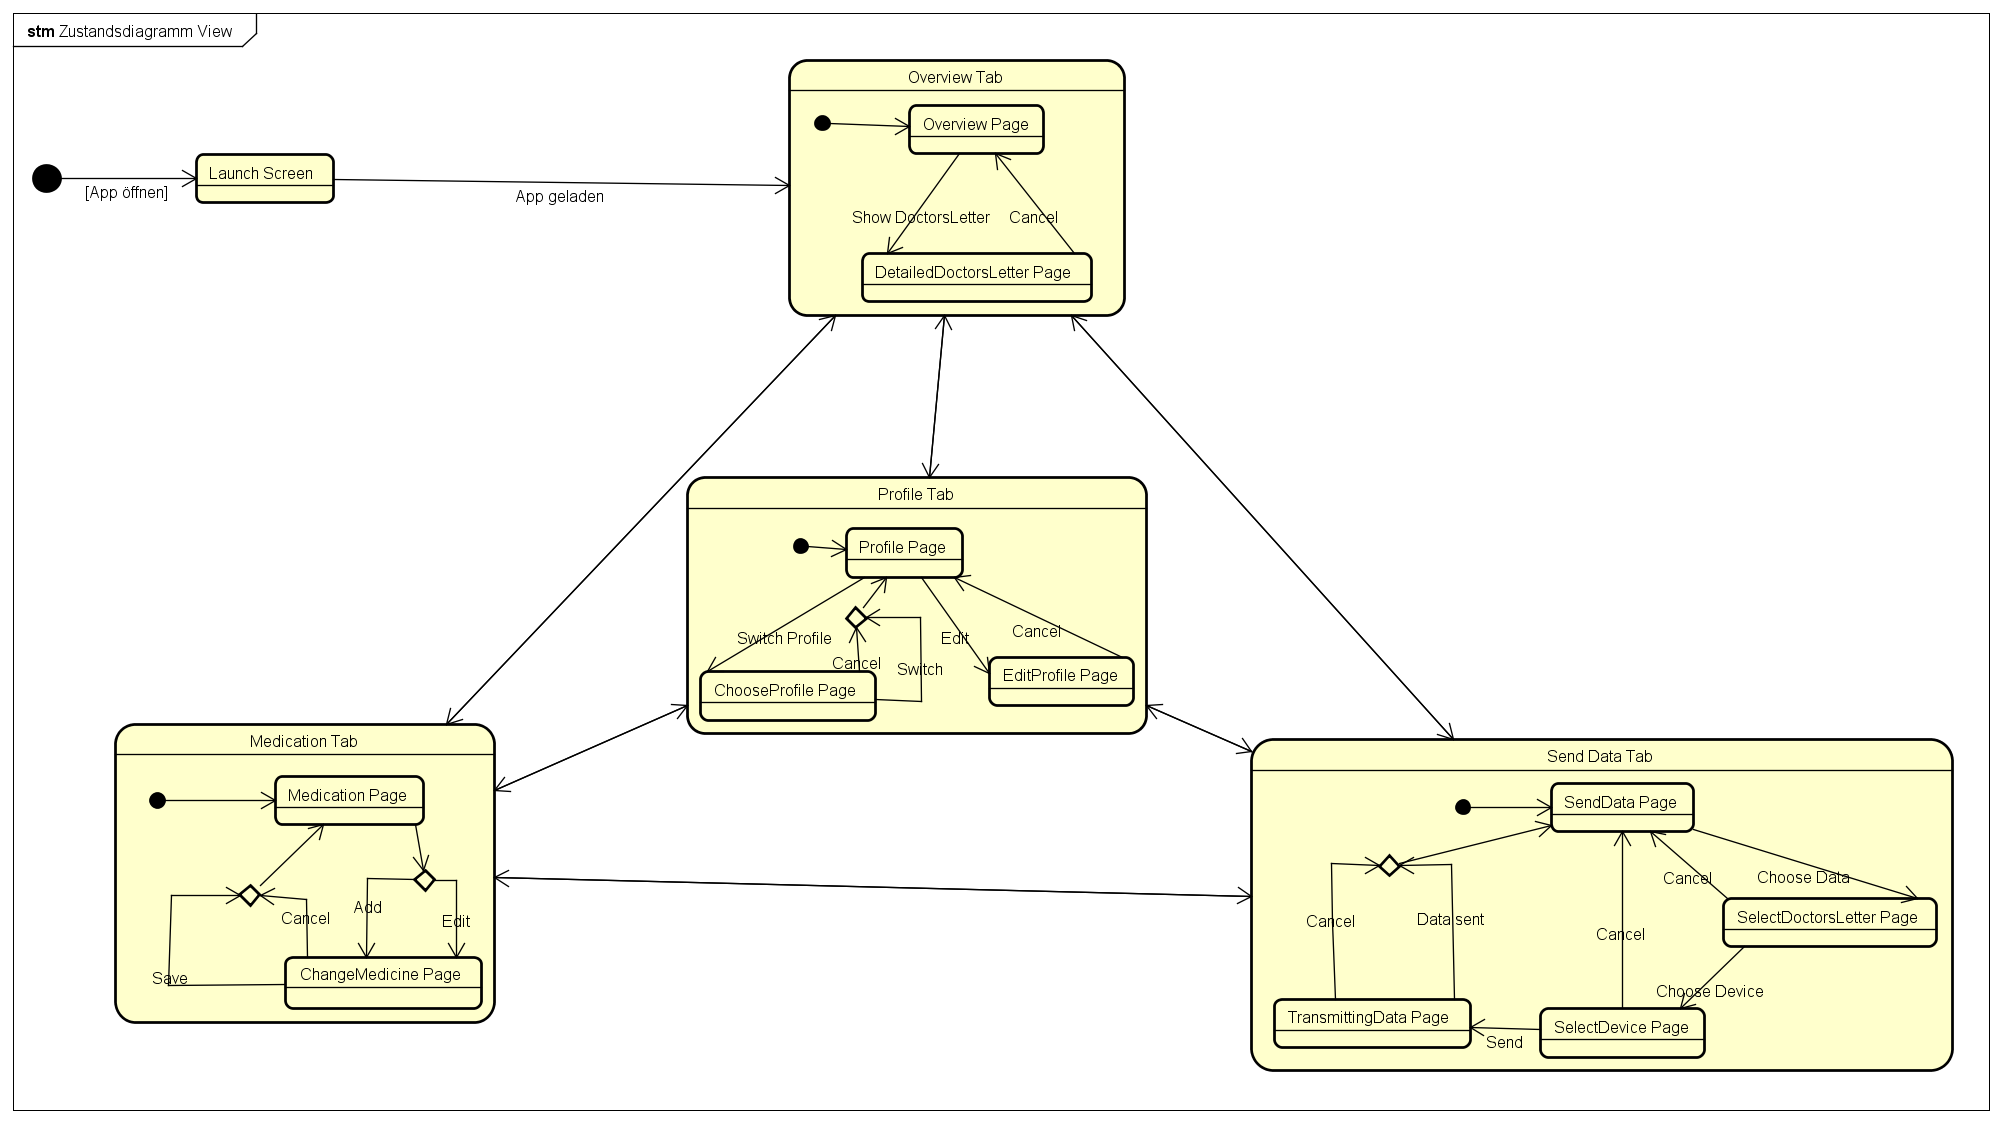
\includegraphics[width=0.9\textheight, angle=90]{graphics/Zustandsdiagramm_View}
\caption{Zustandsdiagramm der View}
\end{figure}
\begin{figure}
Die hauptsächliche Navigation in der Anwendung erfolgt über eine Tab Bar, die es dem Nutzer erlaubt, von jedem der vier Tabs in einen beliebigen anderen wechseln zu können. 
\\
\\
Startet der Nutzer die Anwendung zum ersten Mal, so gelangt er nach einer Begrüßung durch den Launch Screen zunächst in den Overview Tab.
Hier bietet sich ihm nun die Möglichkeit, durch das Auswählen eines beliebigen Arztbriefes in eine detaillierte Ansicht des Briefes zu gelangen.
Von hieraus gelangt der Nutzer nur durch einen Klick auf den Schließen Knopf zurück zur Overview Page.
\\
\\
Wechselt der Nutzer nun in den Medication Tab, gelangt er zunächst in die Medication Page. Diese stellt eine Übersicht über alle eingetragenen Medikationen dar. Über einen Hinzufügen Knopf gelangt man von dort aus in die ChangeMedicine Page, die das Anlegen einer neuen Medikation ermöglicht. Mit einem Klicken auf Speichern oder Abbrechen gelangt man wieder zurück zur Medication Page. Eine zweite Möglichkeit, die ChangeMedicine Page zu erreichen, stellt das Tippen auf einen beliebigen Eintrag der MedicationPage dar: Dadurch bietet sich die Möglichkeit, die vorhandenen Werte der Medikation anzupassen.
\\
\\
Der SendData Tab präsentiert dem Nutzer zunächst die SendData Page, von wo aus ein Tippen auf einen Knopf weiterleitet zur SelectDoctorsLetter Page, die es ermöglicht, die zu übertragenden Arztbriefe auszuwählen. Sind alle Dateien ausgewählt, gelangt der Nutzer über einen Knopf zur SelectDevice Page, wo er einen Empfänger auswählen kann. Hat er auch das erledigt, leitet ihn ein letzter Knopf zur TransmittingData Page weiter, die ihm einen Überblick über den Übertragungszustand bietet. Nach erfolgreicher Datenübertragung gelangt er über einen Knopf zurück zur SendData Page.
Alle der drei genannten Pages verfügung zudem über einen Cancel Button, der den Nutzer direkt zurück zur SendData Page leitet, und beispielsweise den Datenübertragungsvorgang abbricht.
\\
\\
Der letzte der vier Tabs, der Profile Tab, stellt dem Nutzer zunächst das aktuelle Profil in der Profil Page dar. Hier hat der Benutzer nun zwei Möglichkeiten: Entweder er entschließt sich zum Wechsel des aktiven Profils durch einen Knopfdruck Switch Profile, oder er möchte das aktuelle Profil editieren. 
Ersteres leitet ihn weiter zur ChooseProfile Page, wo er aus den gespeicherten Profilen zu einem beliebigen wechseln kann. Ein Speichern Knopf sichert die Änderung und leitet zurück zur Profile Page.
Möchte der Nutzer allerdings ein Profil editieren, erreicht er dies über einen Edit Knopf, der ihn zur EditProfile Page weiterleitet. Hier können entweder die eingetragenen Werte geändert und durch einen Speichern Knopf gesichert werden, oder durch man bricht den Vorgang durch einen Cancel Knopf ab. Beides leitet den Nutzer zurück zur ProfilePage.
\\
\\
Die Anwendung lässt sich zu jedem Zeitpunkt beenden. Aktive Datenübertragungsvorgänge werden dadurch jedoch beendet. Zudem gehen nichtgespeicherte Änderungen jeglicher Art verloren.
\end{figure}

\begin{figure}
\section{UI-Seiten}

% Overview Tab Page
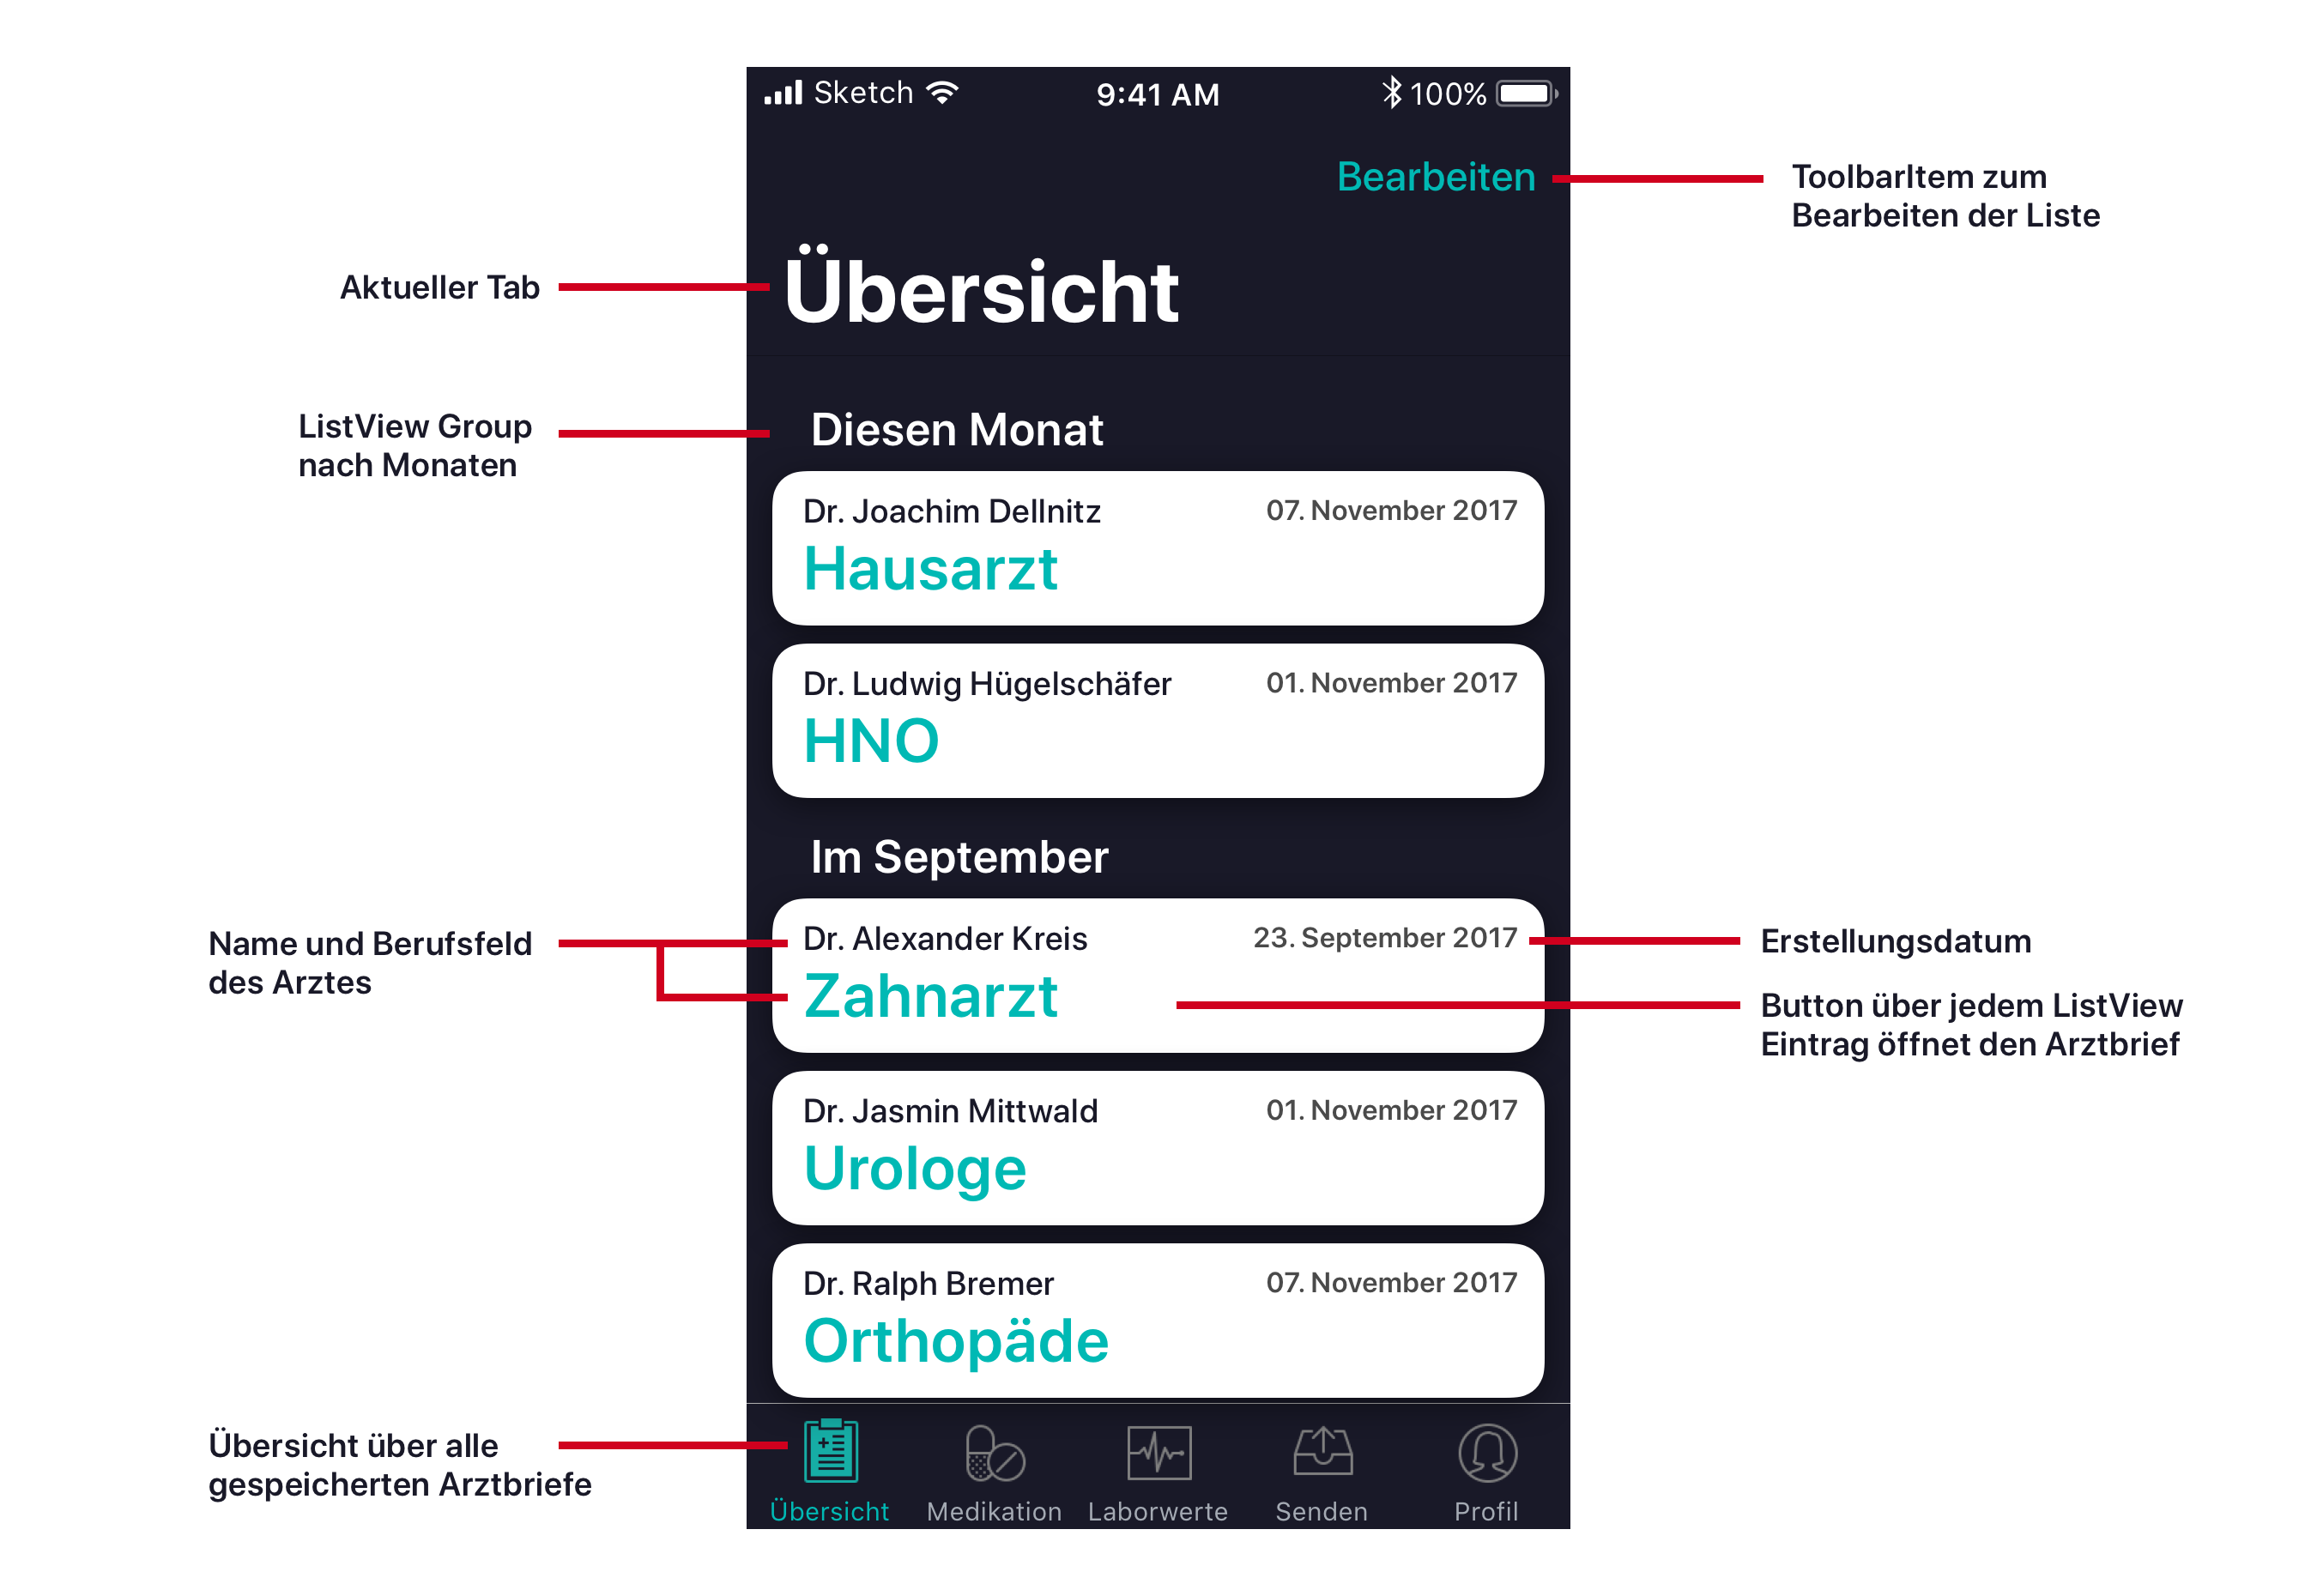
\includegraphics[width=1\textwidth]{graphics/UIDescriptions/OverviewDesc}
\caption{Beschreibung des Tabs "Übersicht"}
\vspace{0.5cm}
Wird die Anwendung geöffnet, wird dem Nutzer zunächst eine Übersicht all seiner gespeicherten Arztbriefe angezeigt (Overview Page). Die Arztbriefe sind hierbei chronologisch absteigend in einer ListView angeordnet. Tippt der Nutzer einen Listeneintrag an, öffnet sich eine ausführliche Ansicht des Arztbriefes.
\end{figure}

% Detailed Doctors Letter Page
\begin{figure}
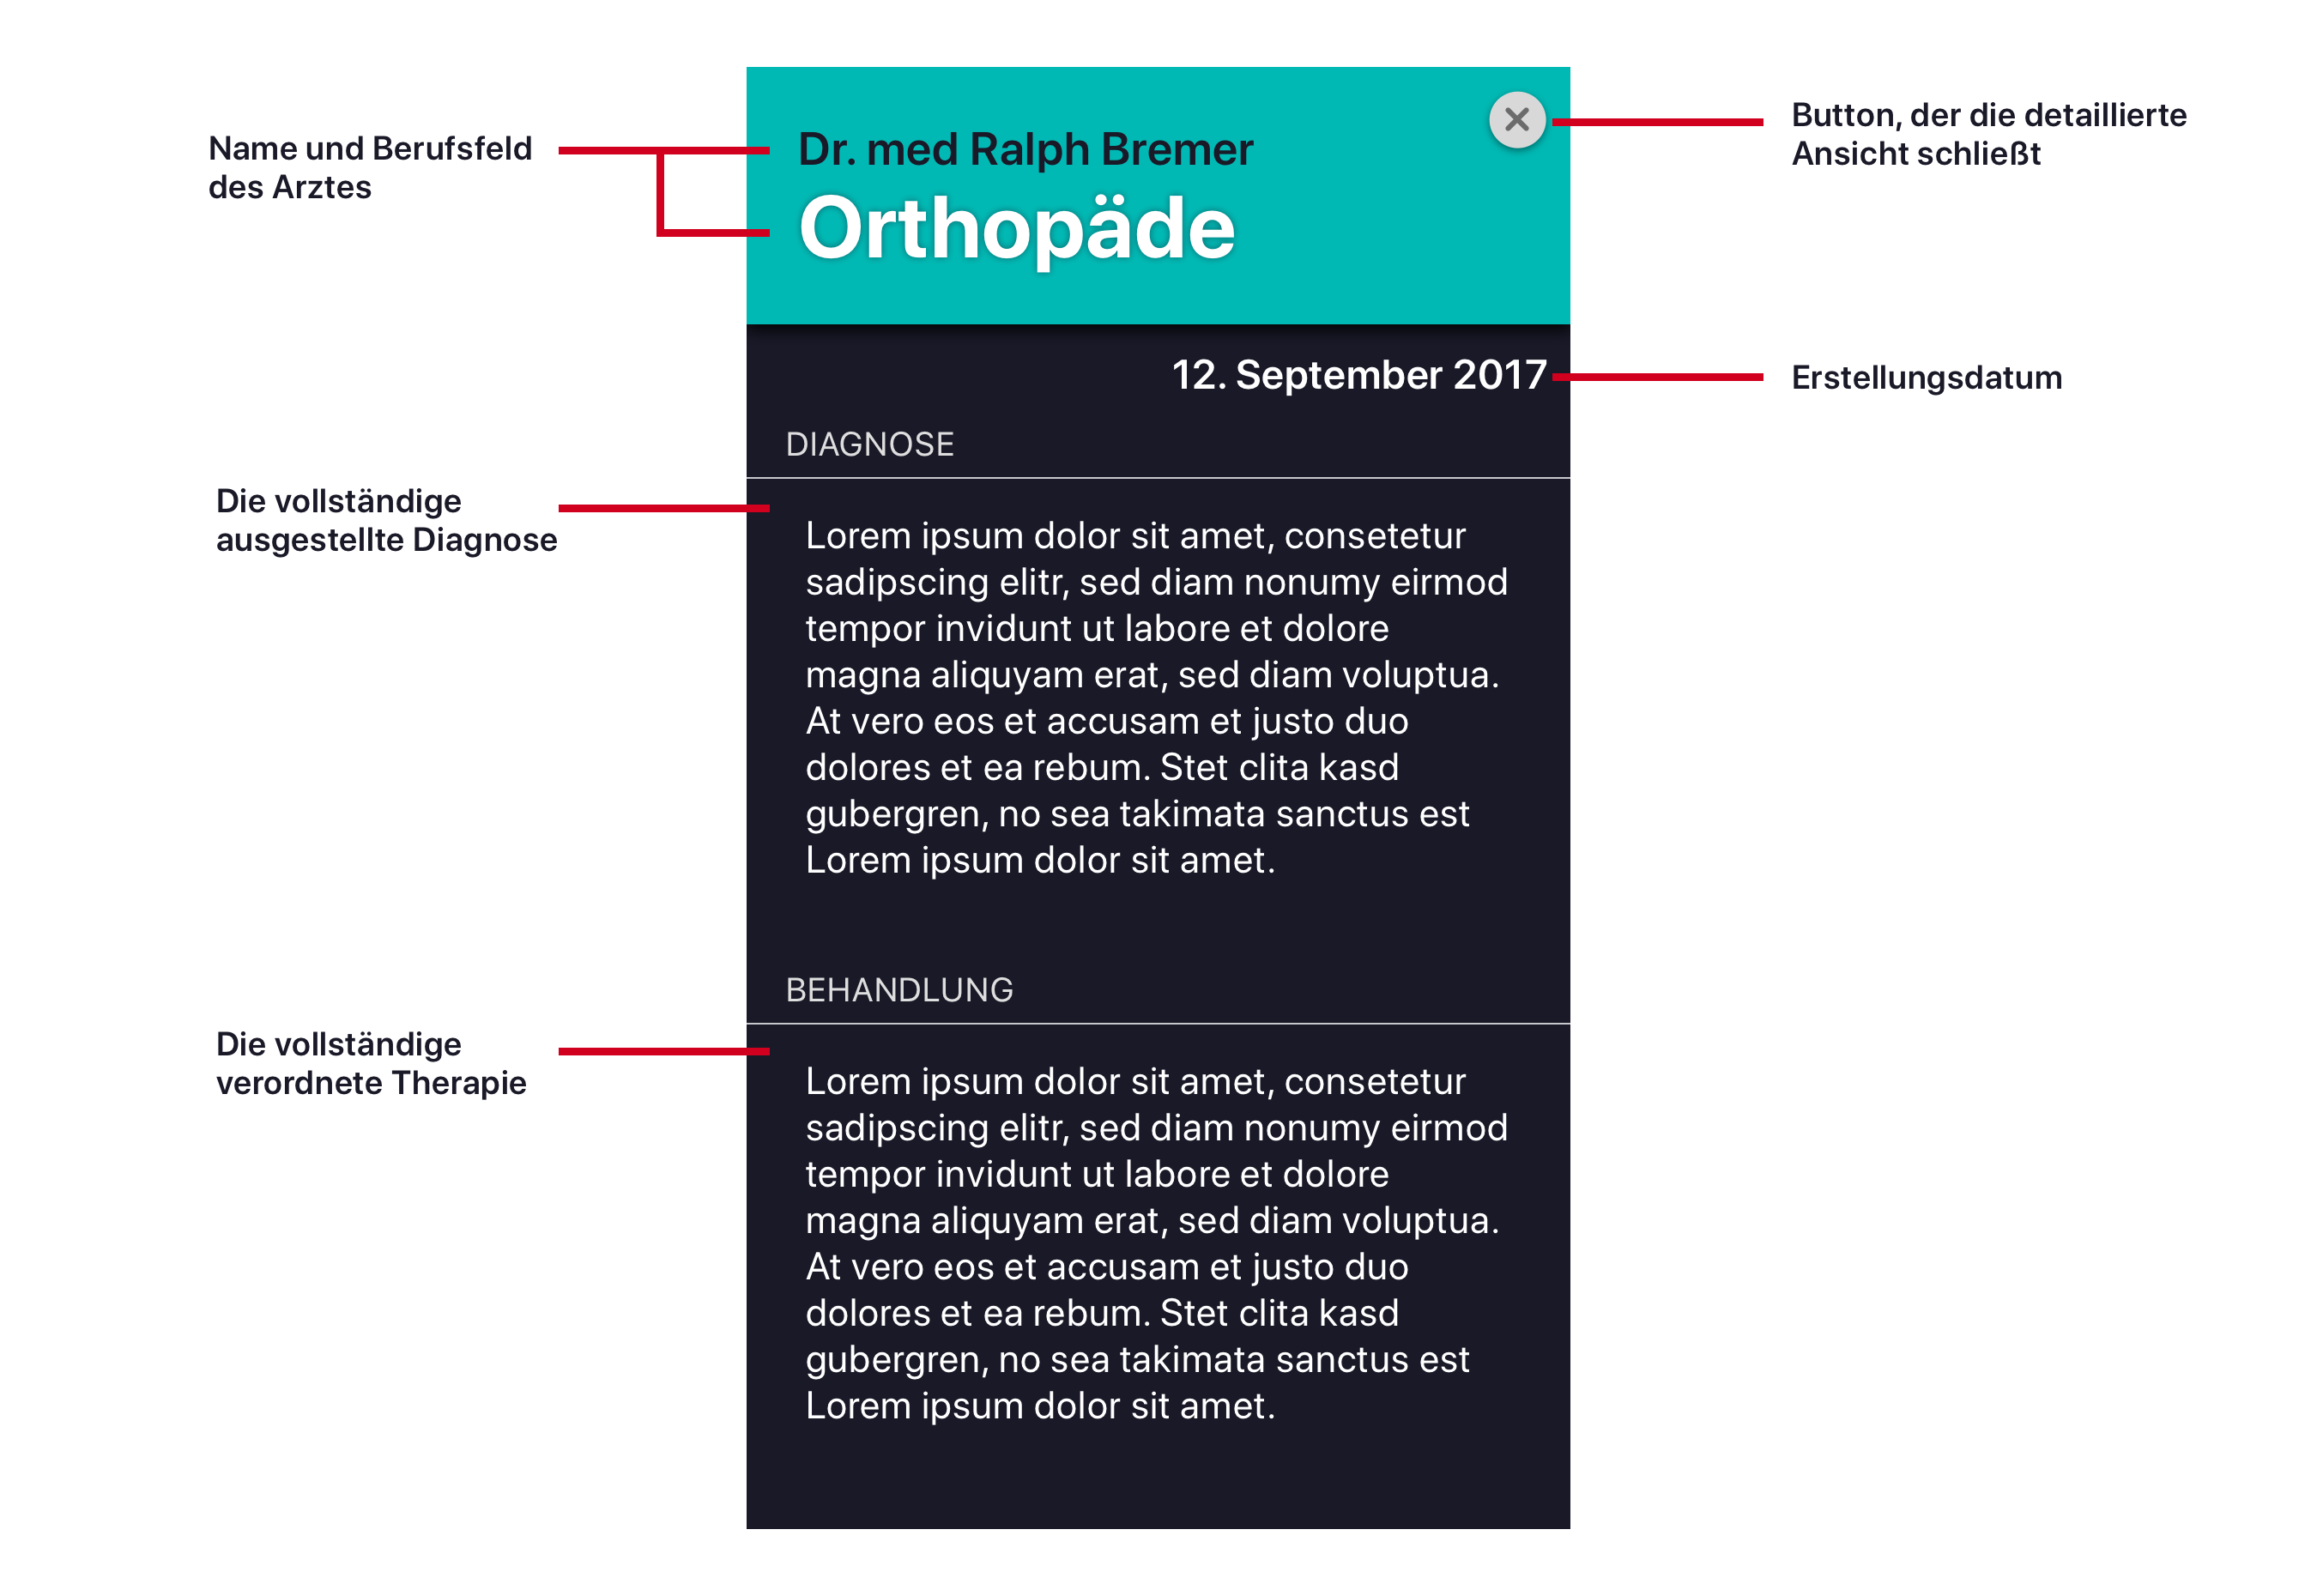
\includegraphics[width=1\textwidth]{graphics/UIDescriptions/DetailedDLDesc}
\caption{Beschreibung der detaillierten Ansicht eines Arztbriefes}
\vspace{0.5cm}
Tippt der Nutzer einen Arztbrief in der Übersicht an, wird er auf eine detaillierte Darstellung des Arztbriefes weitergeleitet. Hier werden, neben dem Datum, dem Namen und Fachrichtung des Arztes, die hinterlegten Daten der Diagnose und der Behandlung vollständig angezeigt. Zum Schließen einer Detailansicht des Arztbriefes, kann der Nutzer auf den \dq Schließen\dq{} Knopf drücken und wird dann zur Übersicht geleitet.
\end{figure}

% Medication Page
\begin{figure}
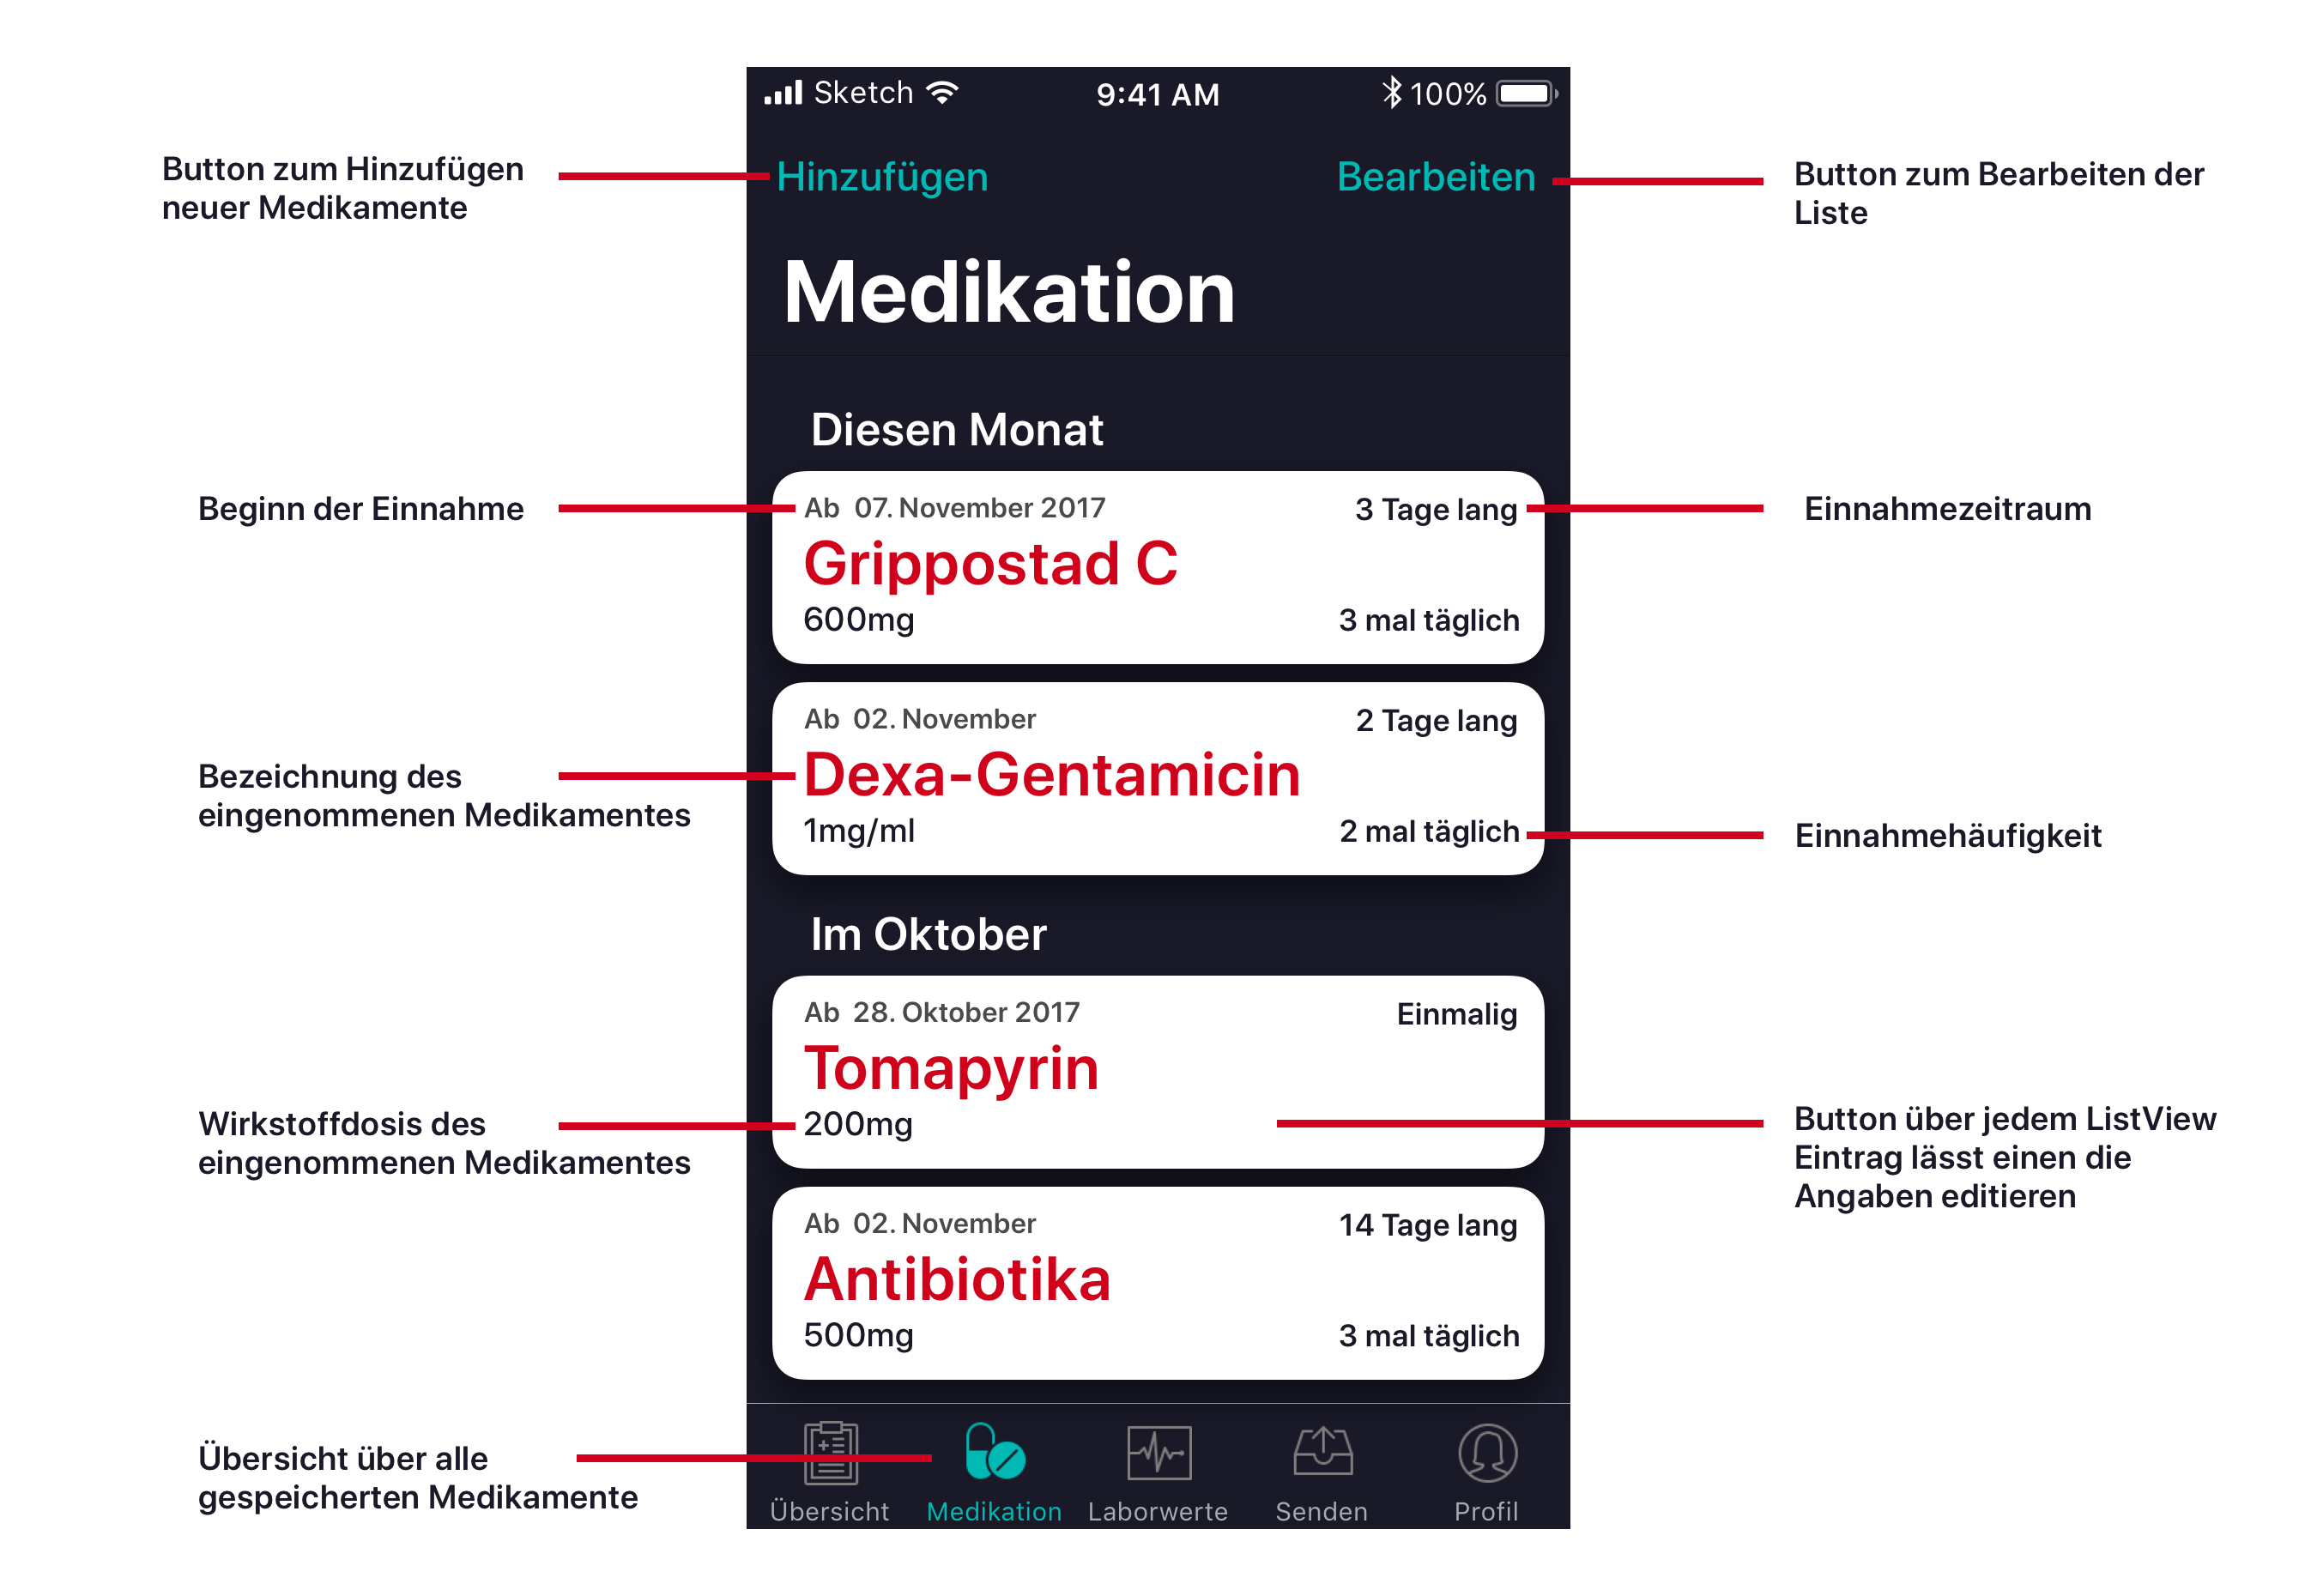
\includegraphics[width=1\textwidth]{graphics/UIDescriptions/MedicationsDesc}
\caption{Beschreibung des Tabs \dq Medikation\dq{}}
\vspace{0.5cm}
Im Tab \dq Medikation \dq{} kann der Nutzer eine Liste von eingenommenen/einzunehmenden Medikamenten verwalten. Dabei wird jeder Eintrag (Medikament) mit allen hinterlegten Daten chronologisch absteigend angezeigt. Um einen Eintrag zu editieren, kann der Nutzer einen Eintrag antippen.
\end{figure}

\begin{figure}
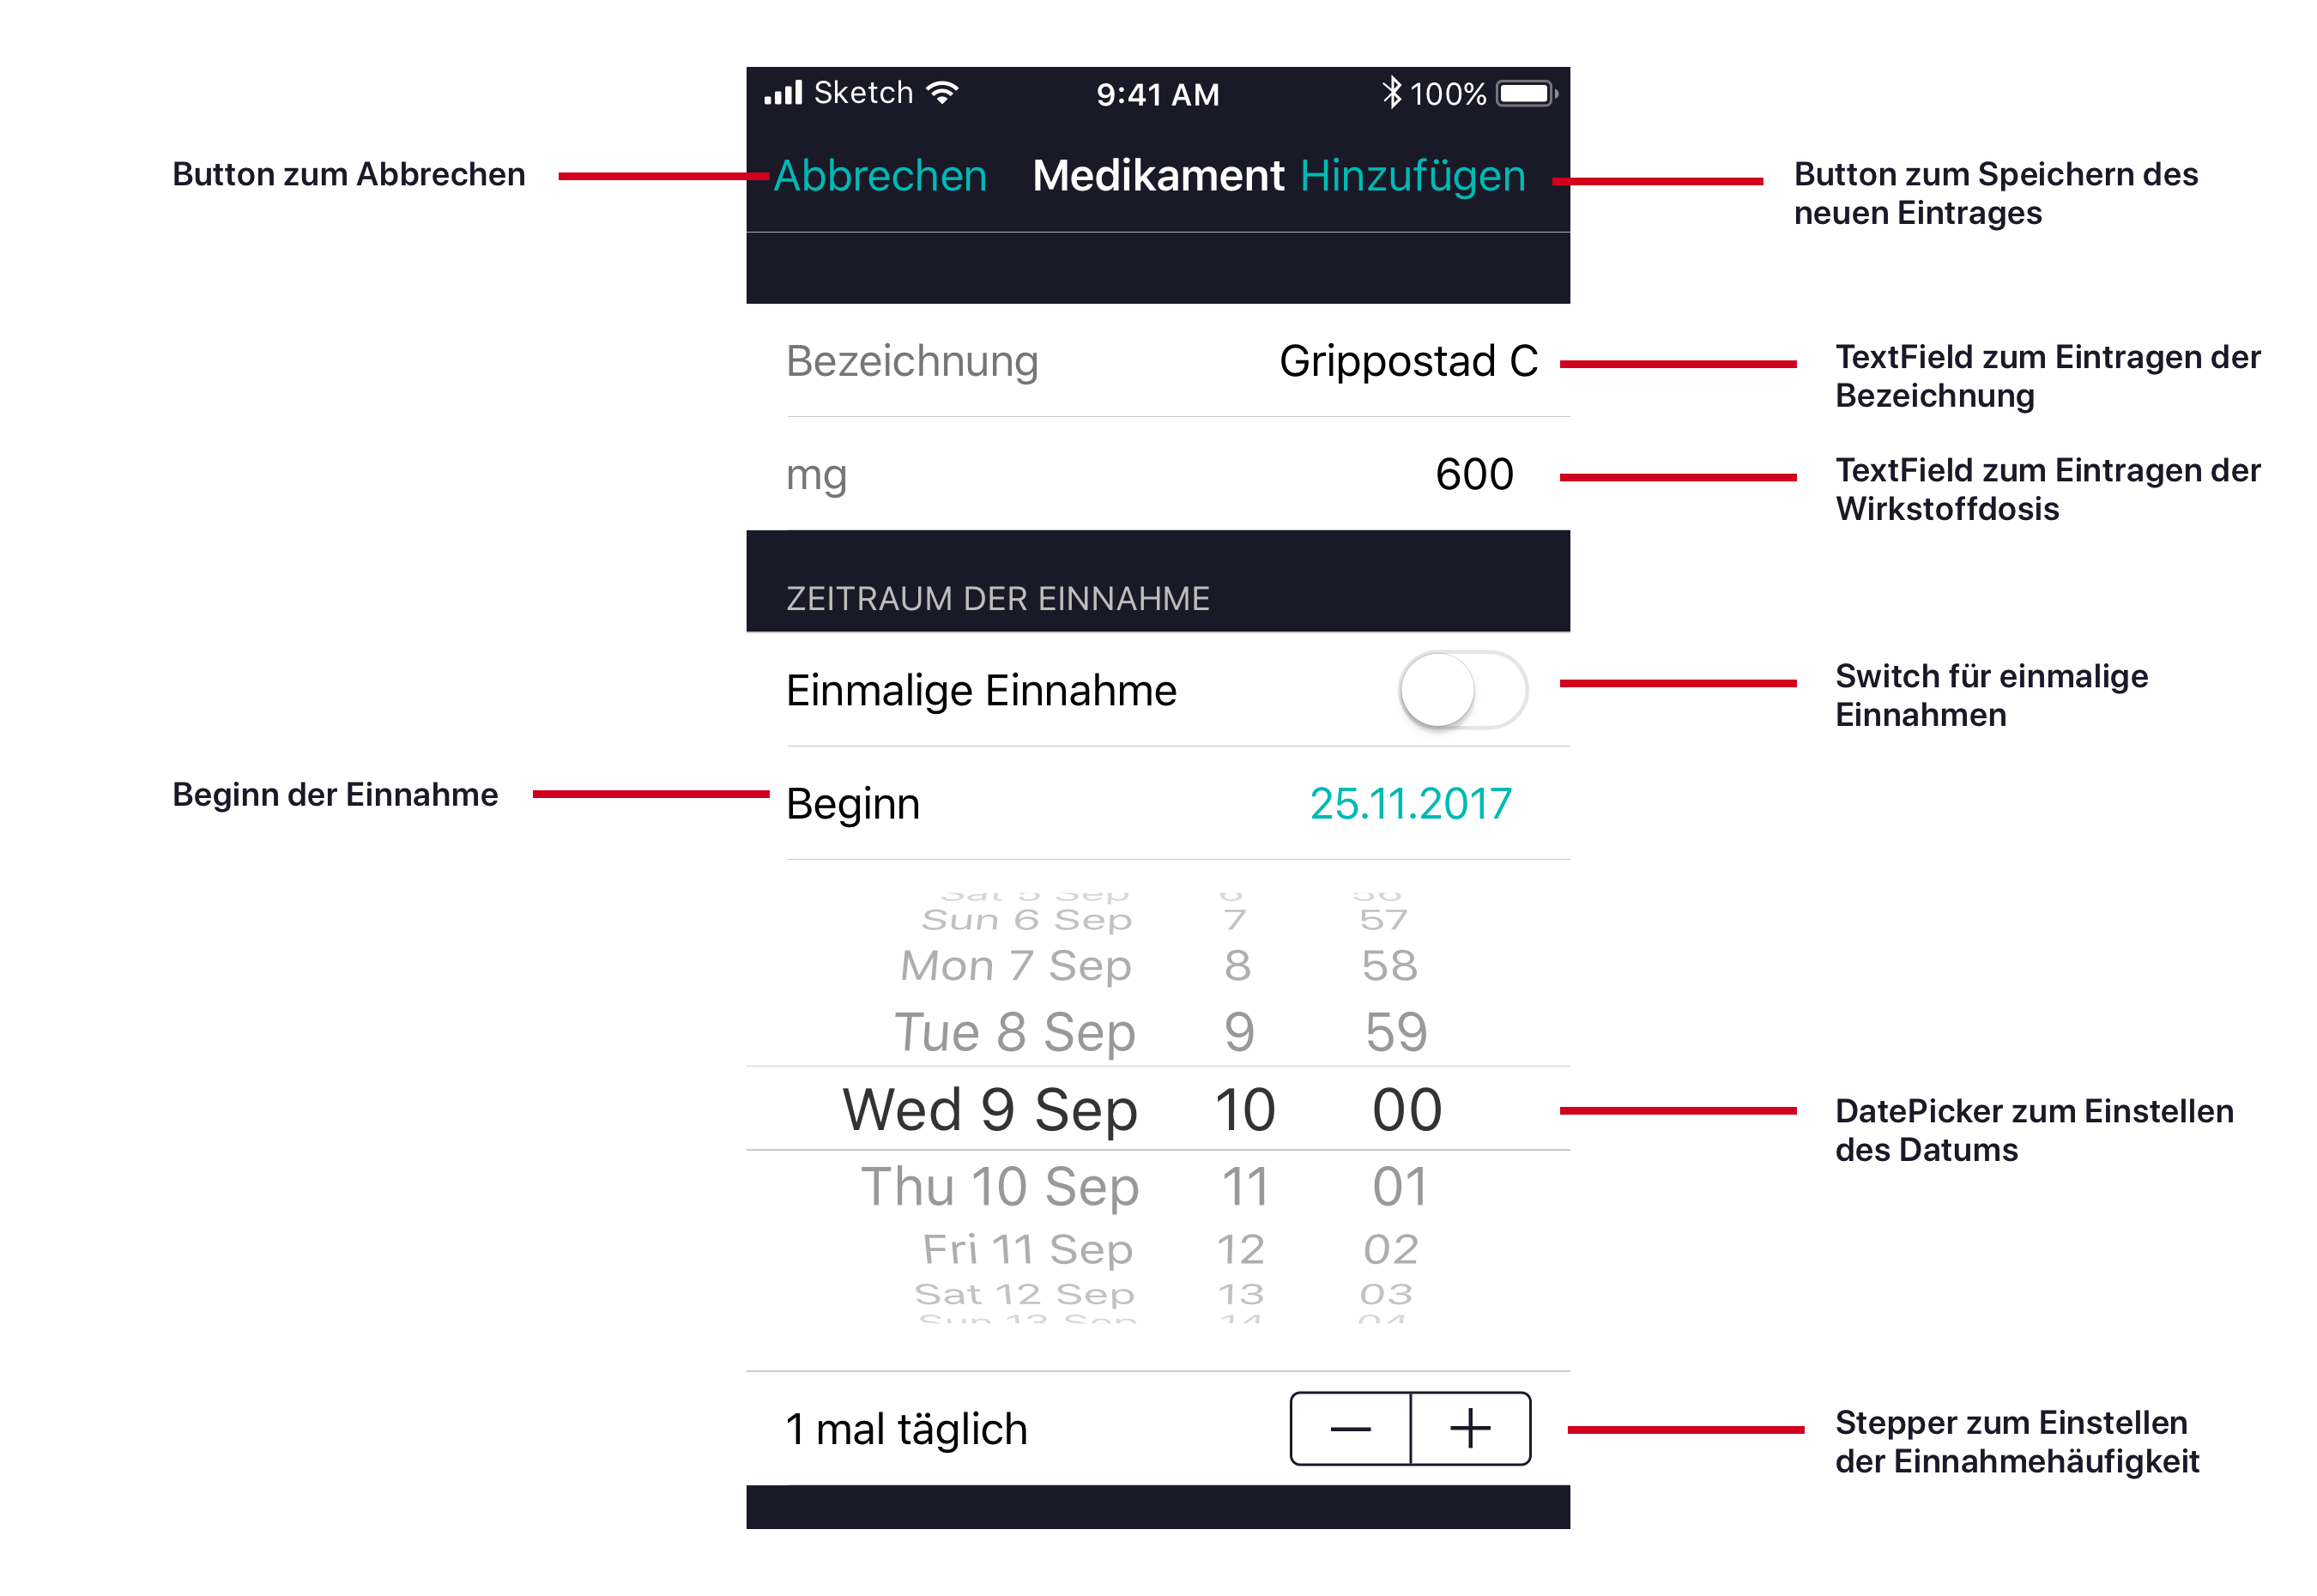
\includegraphics[width=1\textwidth]{graphics/UIDescriptions/DetailedMedicationDesc}
\caption{Beschreibung der Ansicht zum Editieren einer Medikation}
\vspace{0.5cm}
In dieser Ansicht lassen sich alle Daten zu einem Medikament editieren. Der Nutzer gelangt in diese Ansicht, indem er entweder ein neues Medikament hinzufügt oder ein bereits bestehendes Medikament editiert. Sobald der Nutzer alle Werte eingetragen hat, kann er auf den \dq Hinzufügen\dq{} Button tippen, um seine Eingabe/Änderung zu speichern. Falls der Nutzer seine Eingabe jedoch nicht speichern möchte, kann er auf den \dq Abbrechen\dq{} Button tippen, um ohne eine Datenspeicherung wieder zurück in den \dq Medikation\dq{} Tab zu gelangen.
\end{figure}

\begin{figure}
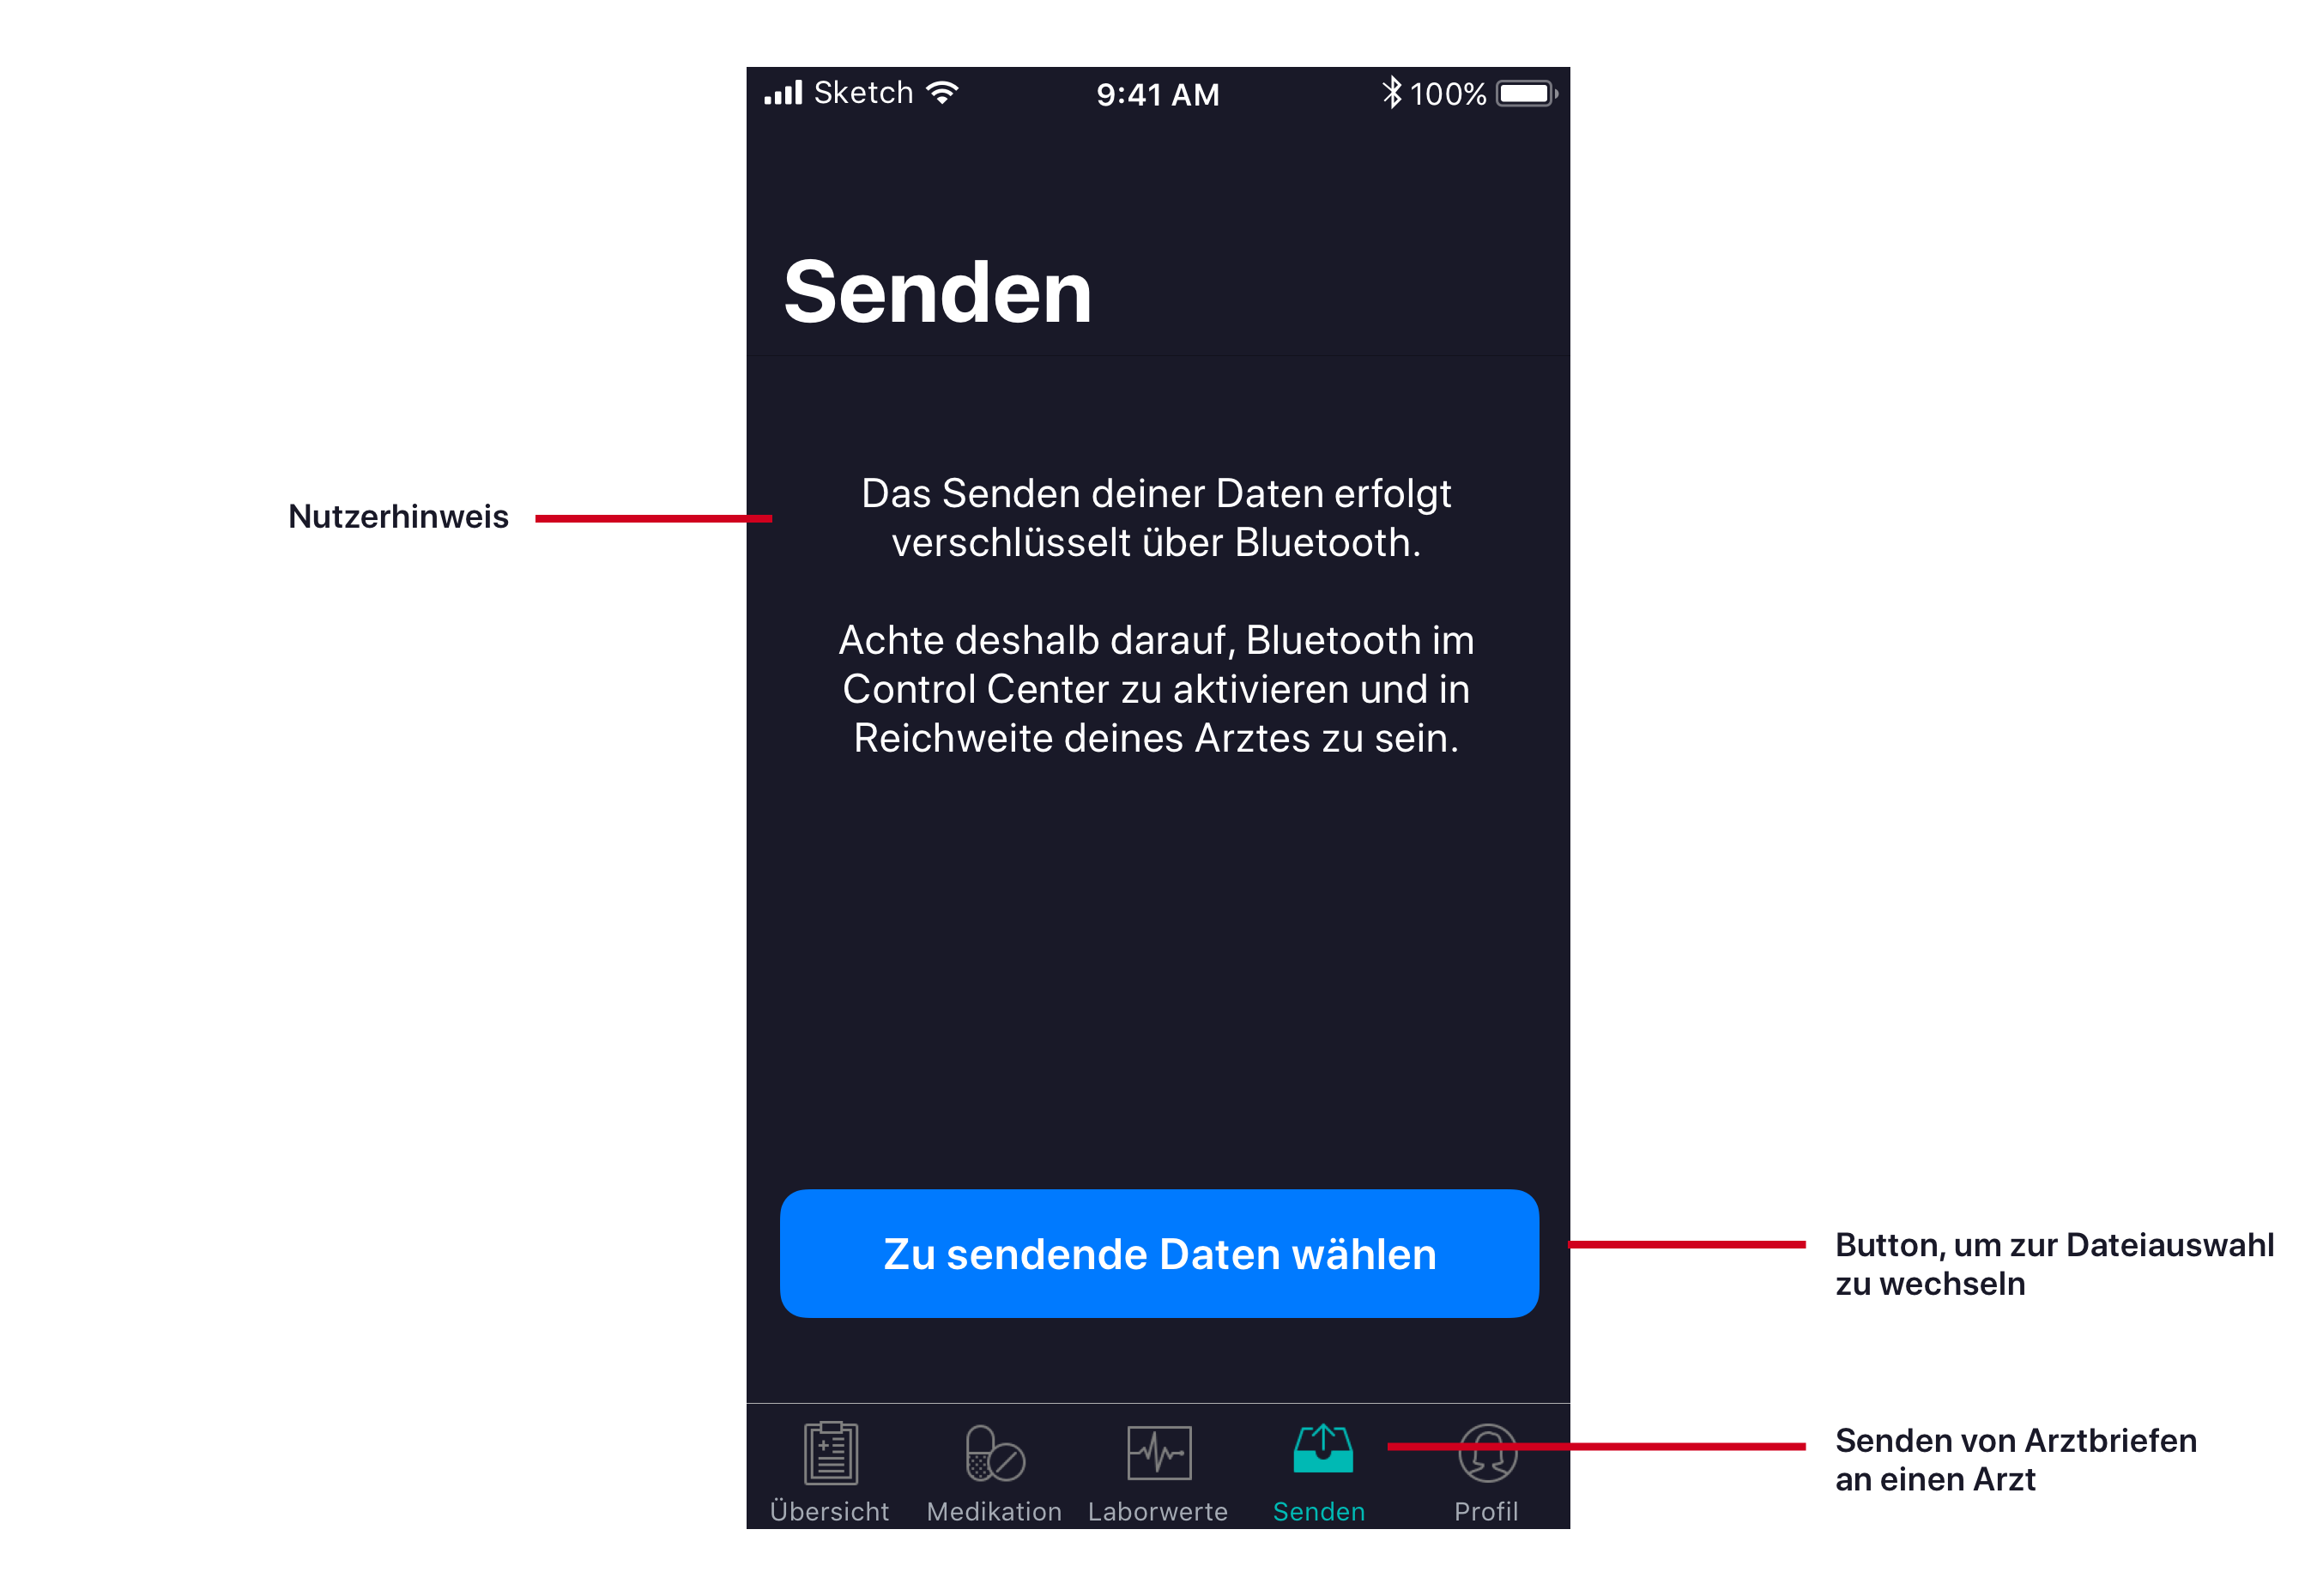
\includegraphics[width=1\textwidth]{graphics/UIDescriptions/SendDataDesc}
\caption{Beschreibung des Tabs \dq Senden\dq{}}
\vspace{0.5cm}
Tippt der Nutzer auf den \dq Senden\dq{} Tab wird ihm ein Nutzerhinweis zur Datenübertragung und ein Button, der zur Dateiauswahl für einen Sendeprozess weiterleitet, angezeigt.
\end{figure}

\begin{figure}
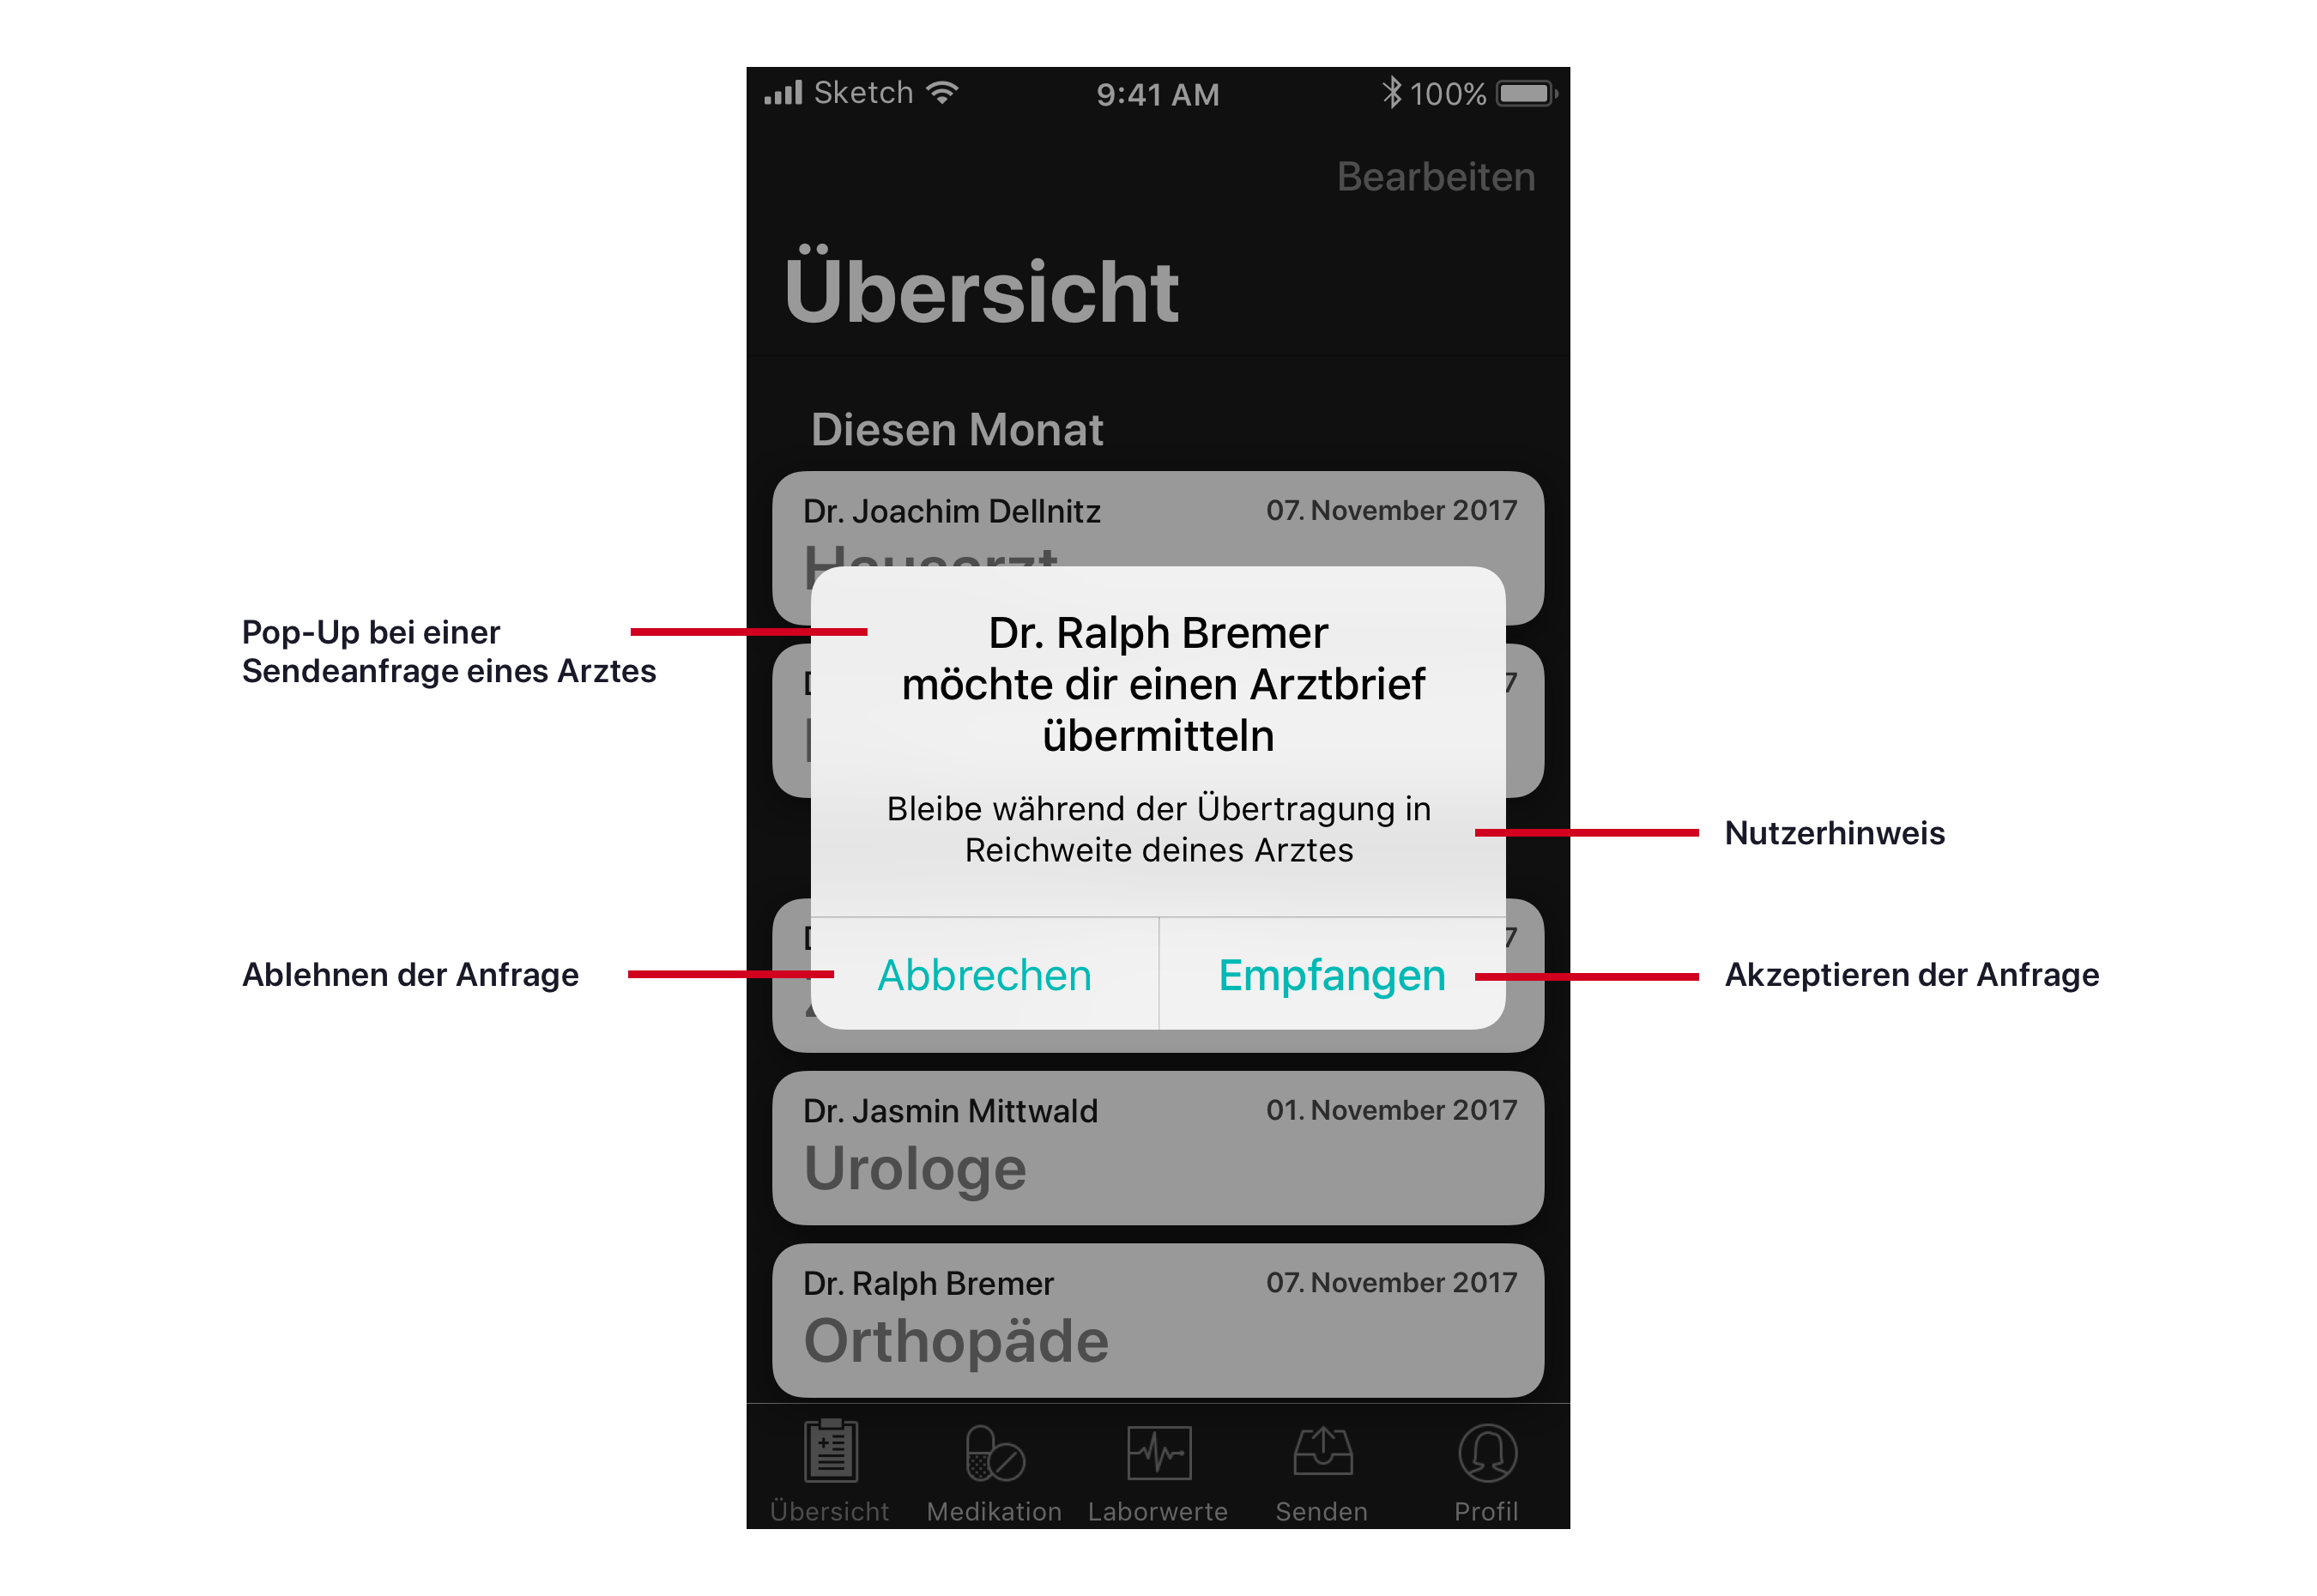
\includegraphics[width=1\textwidth]{graphics/UIDescriptions/PopUpDesc}
\caption{Beschreibung der Ansicht einer Sendeanfrage}
\vspace{0.5cm}
Die Sendeanfrage wird durch ein Pop-Up Fenster realisiert. Das Pop-Up kann in jeder Ansicht erscheinen. In dem Pop-Up wird der Name des Senders, ein Nutzerhinweis und zwei Buttons angezeigt. Es gibt einen \dq Abbrechen\dq{} Button und einen \dq Empfangen\dq{} Button. Tippt der Nutzer den\dq Abbrechen\dq{} Button an, wird die Sendeanfrage abgelehnt und es findet keine Datenübertragung statt. Tippt der Nutzer jedoch den \dq Empfangen\dq{} Button an werden die Daten vom Sender an den Nutzer übertragen.
\end{figure}

\chapter{Anwendung für Ärzte}
Die Version der Anwendung die nicht von Patienten, sondern von Ärzten verwendet werden soll um Patienten deren Arztbriefe zu senden, wird in diesem Dokument nicht genauer beschrieben, da sie nur eine reduzierte Version der hier beschriebenen mobilen Anwendung ist. 

Die Anwendung für Ärzte soll nur Dateien mit mobilen Anwendungen von Patienten austauschen können, also
sind dort die Pakete für die Modellierung (\textbf{DataModel}, \textbf{EntityFactory}), Speicherung (\textbf{DatabaseModel}, \textbf{EntityObserver}) der Daten überflüssig. 

Somit wird auch die Logik zur Konvertierung zwischen den Speicherungsformaten (\textbf{ParserModel}) nicht mehr benötigt. 

Weiterhin werden die gesendeten/empfangenen Dateien nicht im Dateisystem der Anwendung, (was die Funktion des \textbf{FileHelper} war), sondern an einem beliebigen Dateipfad gespeichert.

Somit ist die einzige für diese Anwendung nötige Funktionalität im Model komplett in \textbf{TransmissionModel} enthalten.

%TODO View, ViewModel je nachdem ob ihr was dazu entworfen habt oder nicht, kommt des halt hier rein oder an den entsprechenden anderen Stellen.

\chapter{Klassendiagramm}
%TODO


\printnoidxglossaries

% Abbildungsverzeichnis
\listoffigures
 
\end{document}
